%%
%% This is file `mcmthesis-demo.tex',
%% generated with the docstrip utility.
%%
%% The original source files were:
%%
%% mcmthesis.dtx  (with options: `demo')
%%
%% -----------------------------------
%%
%% This is a generated file.
%%
%% Copyright (C)
%%     2010 -- 2015 by Zhaoli Wang
%%     2014 -- 2016 by Liam Huang
%%     2016 -- 2018 by Xuehan Sun
%%
%% This work may be distributed and/or modified under the
%% conditions of the LaTeX Project Public License, either version 1.3
%% of this license or (at your option) any later version.
%%
%% This work has the LPPL maintenance status `maintained'.
%%
%% The Current Maintainer of this work is Xuehan Sun.
%%
\documentclass{mcmthesis}
\mcmsetup{CTeX = false,   % 使用 CTeX 套装时,设置为 true
        tcn = 011, problem = B,
        sheet = true, titleinsheet = true, keywordsinsheet = true,
        titlepage = true}
\usepackage{amsmath, amssymb}
\usepackage{mathrsfs}
\usepackage{palatino}
\usepackage{mwe}
\usepackage{graphicx}
\usepackage{subfig}
\usepackage{subcaption}
\usepackage{float}
\usepackage{multirow}
\usepackage{indentfirst}
\usepackage{gensymb}
\usepackage[ruled,lined,commentsnumbered]{algorithm2e}
\usepackage{geometry}
\usepackage{pdfpages}
\usepackage{array}
\usepackage{verbatim}
\geometry{left=2cm,right=2cm,top=2cm,bottom=2cm} %%页边距

\begin{document}

\linespread{0.6} %%行间距
\setlength{\parskip}{0.5\baselineskip} %%段间距
\title{BusHub: Guarantee for Quick Home}

\date{\today}
	\begin{abstract}
	
     Located about thirty kilometres east of the city center, Pudong Airport
     occupies a 40-square-kilometre site adjacent to the coastline
     in eastern Pudong. After years of growth on its passenger throughput and expansion of its site, though, Pudong Airport seems to let down its red-eye flight passengers in the aspect of weak evacuation capacity  at midnight.
     
     To address this unsatisfactory situation, our paper establishes the foundation of a bus booking platform, BusHub, which efficiently relieve the backlog of passengers off board, and reduces their waiting duration for commuting. We propose three models, Destination Selection Model, Route Selection Model, and Bus dispatching Model, to offer real-time flexible route planning as well as order dispatching. Meanwhile, we aim to provide an economic and quick service for passengers, promoting user experience. An app advertisement is also devised for marketing purposes.
     
     Destination Selection Model aims to select potential destinations with Metropolis-Hastings Algorithm(MHA), based on population and transportation density. The final fifty destination stations are selected through K-Means Clustering. 
     
     Route Selection Model use the outcomes of Destinaton Selection Model, and employ Simulated Annealing to finalize our choice of routes.

     The cost function is applied to achieve a better outcome of route planning.
     
     Bus Dispatching Model is aimed at arranging bus schedules properly, to achieve a good balance between platform profits and user satisfaction. We employ the Greedy Algorithm and Queueing Theory to better support our model theoretically.

	 The profit function is used to get the best bus-dispatching strategies.
	 
	 To collect enough accurate data, we surveyed the statistical yearbook, literature and other resources. This gives our model a decent input.
	
	 Afterwards, we make sensitivity analysis and discuss our model's strengths and weaknesses.
	 
	 In the end, we come up with an advertisement to promote our app: BusHub.
	
		\begin{keywords}
		destination selection; route selection; cost; profit; user satisfaction; BusHub
		\end{keywords}
	\end{abstract}

\maketitle
\tableofcontents
\newpage

\section{Introduction}
\subsection{Restatement of the Problem}
Constructed in the late 1990s, Shanghai Pudong International Airport is one of two international airports of Shanghai and a major aviation hub of China. Pudong Airport mainly serves international flights.

\begin{figure}[h]
    \centering
    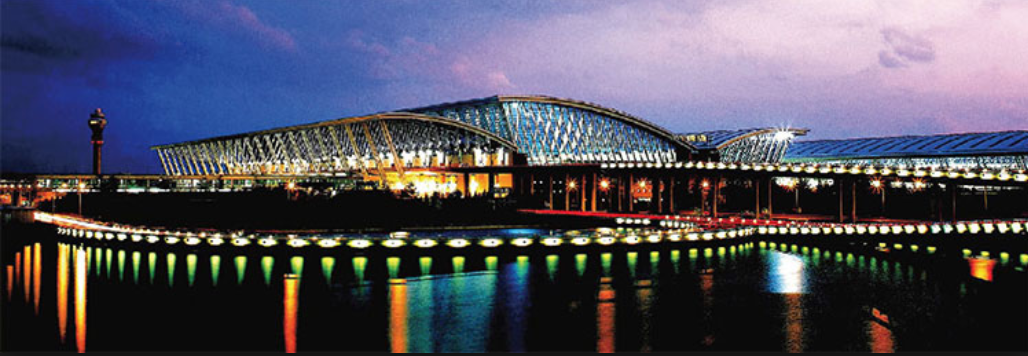
\includegraphics[width=0.8\textwidth]{SPIA.png}
    \caption{Shanghai Pudong International Airport \cite{Google_SPIA}}
    \label{fig:SPIA}
\end{figure}

As a huge rendezvous for many passengers, Pudong Airport has put forward a large number of measures to evacuate passengers, such as the famous maglev, underground, and shuttle buses. This operates quite well during daytime. However, during midnight period(23:00-02:00) when travellers get off from the red-eye flight, there's simply not enough transport capabilities to ensure passengers arrive at their destination in a short time. According to official statistics from Shanghai Traffic Management Bureau(STMB), around 10,000 passengers are stranded at the airport, waiting for a home-ride for a long duration.

Thanks to the overwhelming trend of the Internet, some novel transportation concepts have been put forward to meet the public's demand, such bus service and car-hailing. STMB intends to devise a new bus-booking platform, combining the benefits of both bus service and car-hailing. This new app hopes to achieve a better passenger experience.

\subsection{Our Work}

We named the bus booking platform BusHub.

In our paper, we focus on maximizing platform's marketing profits, promoting user satisfaction, and receiving orders as many as possible.Our model achieves a good balance among them. Destination Selection Model and Route Selection Model generates a reasonable route. Bus Dispatching Model gets a decent bus-departing schedule. 

In Section \ref{sec:assu}, we state four basic assumptions. Section \ref{sec:Nome} is made up of the nomenclature used in the model statement. Section \ref{sec:stat} provides sufficient details about our proposed. Section \ref{sec:impl} implements our model with given and collected data. We conduct several targeting experiments and analyze our model in Section\ref{sec:mode}. At last, we make our conclusions and devise an advertisement for our app in Section \ref{sec:conc} and Section \ref{sec:adve} respectively.

\section{Assumptions}\label{sec:assu}

Our model makes four assumptions as follows:

\begin{enumerate}
	\item In the phase of modeling, we consider each passenger as the same individual subject, and the taxi and bus GPS data on January 31st, 2007 statistically representative. We assume each passenger has the same standard for user satisfaction, namely satisfied if a bus is available while unsatisfied if not. Besides, we suppose there's little difference between the GPS data on the date we choose and others'.
	\item We use plane-coordinate system to replace spherical coordinates. Since Shanghai is not that big if seen from the globe, it is reasonable to assume like this.
	\item The GPS data typically reflects passengers' demands for buses' destinations. Since it's at deep night, there's few traffic jams. Besides, waiting time at the crossroads are randomly equal. 
	\item There is only one starting station, namely the Airport Station, and fifty terminal stations to choose from. All passengers need to go to the airport station to enjoy our bus-booking service. We don't take different airline landing site into account. 
	\item All the buses are the same, and seat 33 people. We simplify the bus to be used as the same standard bus, which has a fixed seat of thirty-three passengers averagely, based on our online research and calculation. Additionally, traffic accidents are ignored because it is rare, especially at night.
\end{enumerate}

\section{Nomenclature}\label{sec:Nome}
In this paper, we use the nomenclature in Table \ref{tab:Nomen} to describe our model. Other symbols that are used only once will be described later in the context.
\begin{table}
    \centering
    \caption{Nomenclature}
    \label{tab:Nomen}
    \begin{tabular}{c c}
\hline
    	Symbol & Definition\\
\hline
	$x$ & The Longitude of each map point\\
	$y$ & The Latitude of each map point\\
	$P(x,y)$ & The Population Density of each map point\\
	$T(x,y)$ & The taxi and bus GPS-recognized position density or Traffic Density\\
	$M(x,y)$ & The Combined Probability Distribution of each map point\\
\hline
    \end{tabular}
\end{table}

\section{Statement of our Model}\label{sec:stat}

In this section, we will discuss our model of predefined route cycles, and how BusHub accept orders. The former model has two major aspects. To begin with, we investigate population density and transportation density of Shanghai to select potential destinations. Then, we provides potential routes for buses, based on selected destinations. This model achieves a great balance between profits and user satisfaction. Profits have many aspects. User Satisfaction is measured according to the number or orders BusHub accept, or in other words, the total number of passengers BusHub transport. Longitude, along with latitude, is replaced by plane coordinates. Besides, Chongmin Island is not taken in account, because it's barely unseen in transportation density chart.

\subsection{Destination Selection Model}

\begin{figure}[h]
    \centering
    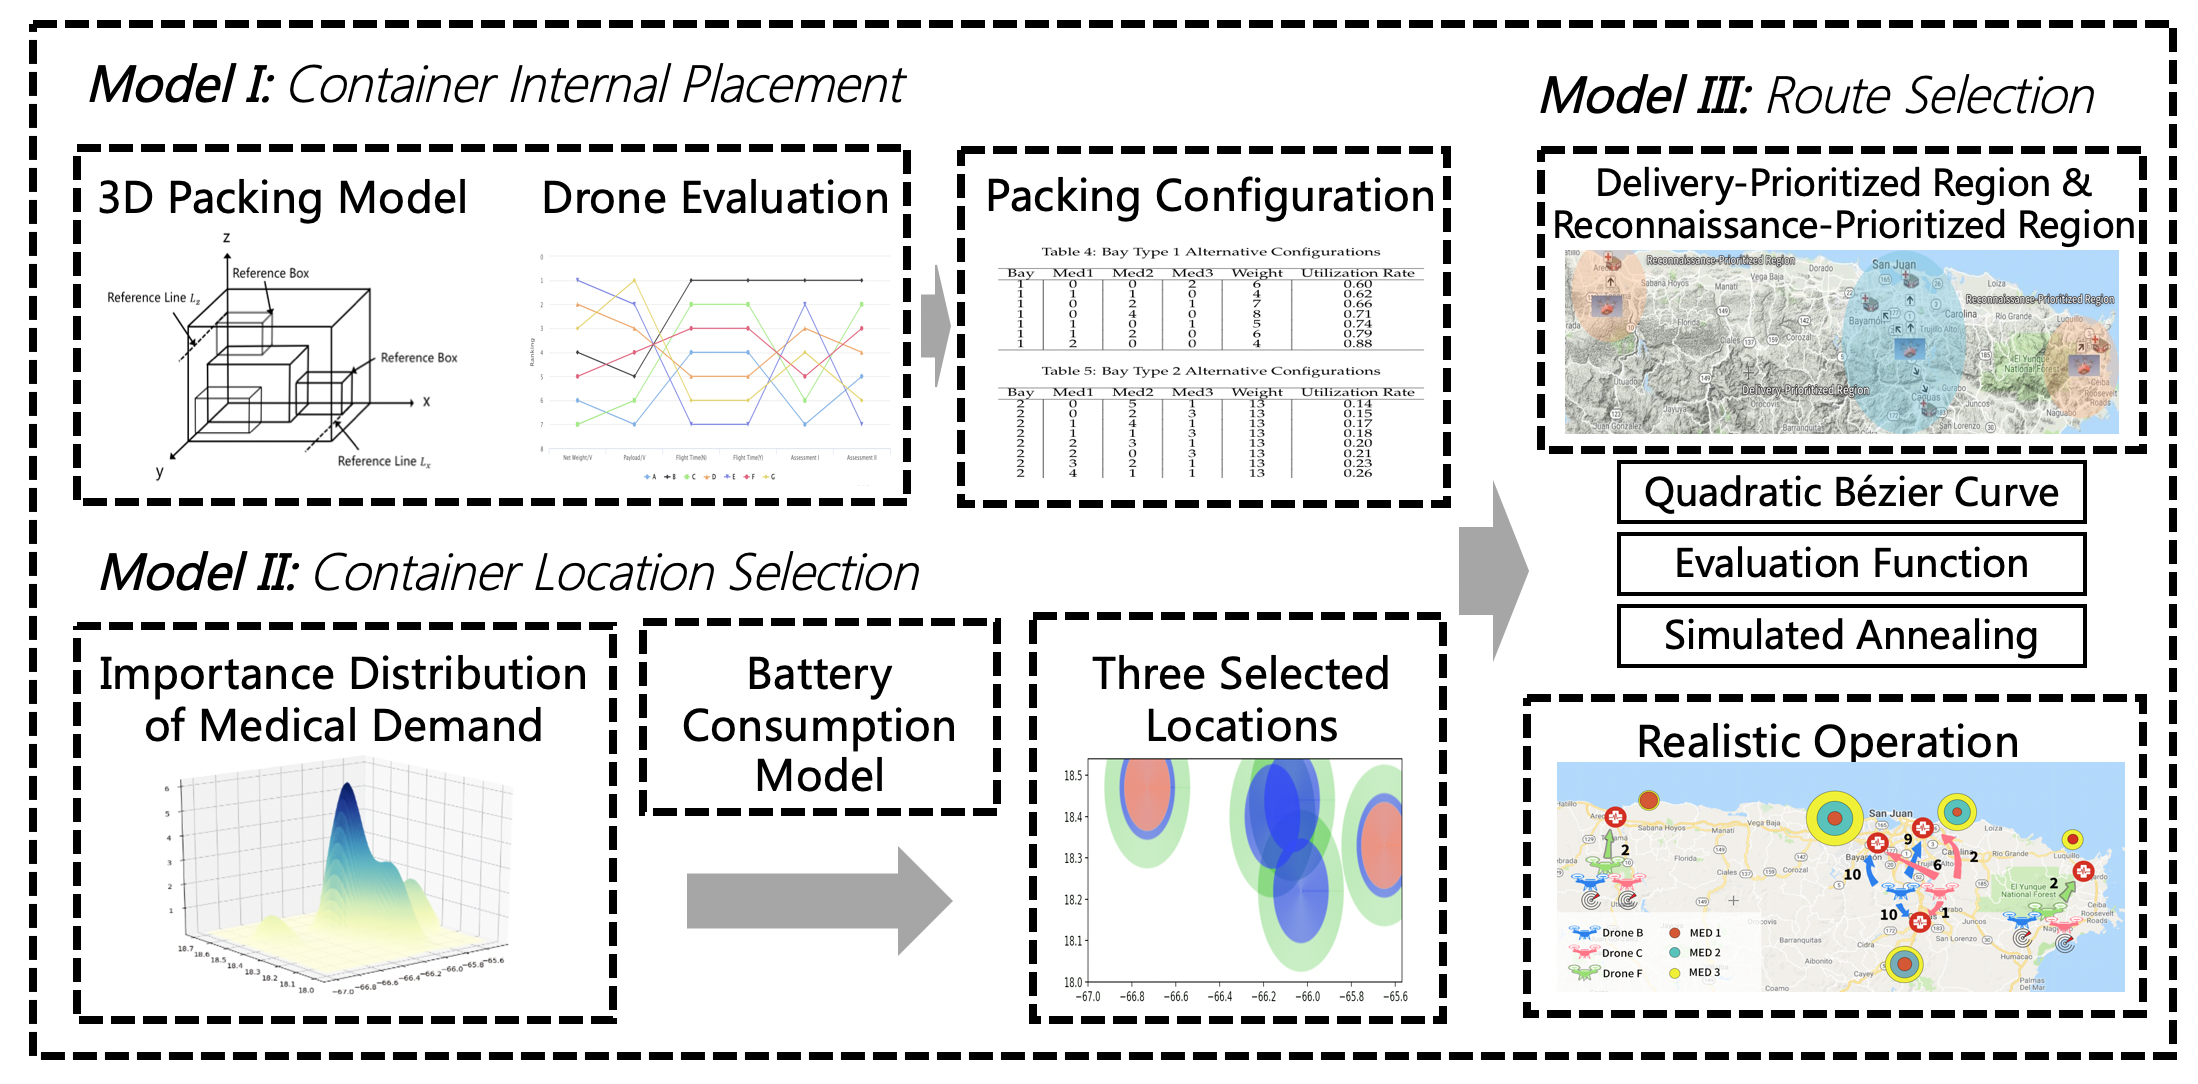
\includegraphics[width=0.8\textwidth]{figures/flowchart.png}
    \caption{Flow Chart of Destination \& Route Selection Model}
    \label{fig:flowchart}
\end{figure}

In our model, we need to select fifty hot destinations for passengers to choose from as their destination station. The population density function $P(x,y)$, and the traffic density $T(x,y)$ are taken into account to form a synthetical destinaiton selection function.

\subsubsection{Destination Selection Function}
In actual situations, for map points with higher population density rate or higher traffic density rate, we are more likely to select these points as our potential destination stations. More people in a certain area means more demands in the region, while more traffic density means people choose to go to these places at that time. 

We use the harmonic mean of $P(x,y)$ and $T(x,y)$ as our final destination selection function $M(x,y)$ to estimate potential destinations probability. This is because the harmonic mean reflects both influence factors evenly. Surely, there are some map points where the traffic density is much higher than population density, but we should take both factors into account, as both matter.

\begin{equation}\label{eq_product&sum}
    M(x,y) = \frac{P(x,y) \times T(x,y)}{P(x,y) + T(x,y)}
\end{equation}

For every map point $(x,y)$, the larger $M(x,y)$ is, the greater possibility for $(x,y)$ to be chosen as a destination. With this formula, we generate a chart on which we can preliminarily see the distribution of potential sites.

\subsubsection{Using Algorithms to Confirm Destinations}
We employ \emph{Metropolis-Hasting Algorithm(MHA)} to sample the function $M(x,y)$, and generate \textbf{potential destinations}. MHA is a Markov Chain Monte Carlo method, which can generate samples of a distribution function proportional to a given function, without normalizing it. Since $M(x,y)$ is a complicated function in two-dimensional space, it's impossible to integrate over the domain. But with MHA, we can still sample this function. Here we obtain a large number of points by MHA to explore where passengers are most likely to arrive at.

Afterwards, \emph{K-Means Clustering} is applied to get reasonable clusters, by which we finalize our selection of \textbf{fifty destination stations}. Additionally, if there are some bad points in them, we can also intervene into the generation of these destinations, but this accounts for only a small part.  In order to satisfy passengers' need as much as possible, we use K-Means to get \emph{k clusters} and set the stations at the heart of \emph{k clusters}. By this, we can \textbf{maximize} the area that buses cover and \textbf{minimize} the average distance between station and passengers' destination. For safety reasons, k is set a little larger than fifty to get rid of undermined bad points.

\subsection{Route Selection Model}\label{sec:rout}

In this section, we firstly introduce concepts related to a route map. Then we analyze factors that could affect the quality of a route map, and define the cost function for a given route map. Finally, we devise an algorithm that could transform samples in primary sample space to a route map, which could be used to find optimal solutions with Simulated Annealing.

\subsubsection{Route Map Concepts}
Based on destinations selected in previous section, we can plan the routes for all the buses. At the very beginning of this section, we'd like to define the concept of a route map. In our model, a route map $\mathscr{R}$ is a tree data structure\cite{TreeStructure}, as presented in Figure \ref{roadmap_demo}. The root node of the tree represents the airport, so we denote it as $V_A$. All the nodes on the tree, except root node and leaf nodes, have only one parent node and one child node. A route $R_i$ is the path from root node to $i$th leave node. Assume that we plan to have $N_R$ routes that depart from the airport, then we have $N_R$ leave nodes in the road map, correspondingly. For each route $R_i$, every vertex $V_{i, j}$(or node in the context of a tree) on the route represents a station, where $j$ is the index of the vertex on that route. Obviously, the airport vertex is the starting vertex of all routes, so $V_{i, 0} = V_A$. Every edge $E_{i, j}$ represents the journey from $V_{i, j-1}$ to $V_{i,j}$. 

\begin{figure}[htbp]
	\centering
	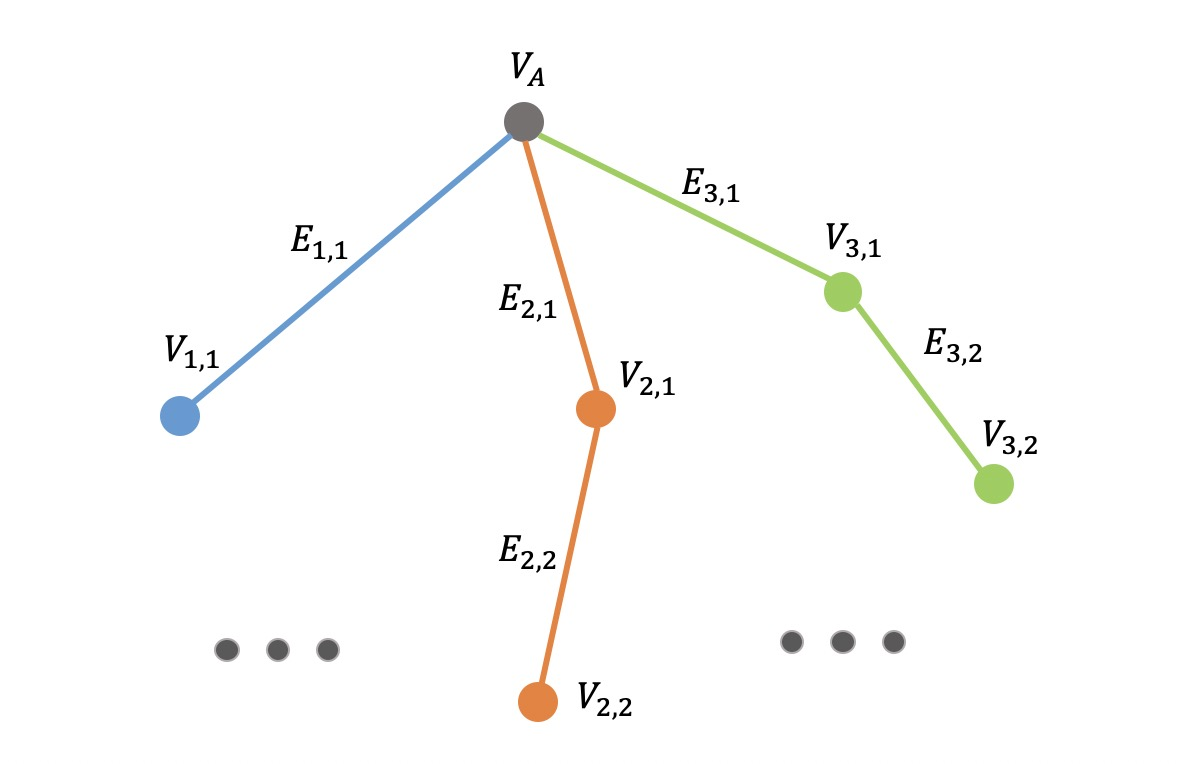
\includegraphics[width=14cm]{figures/routedemo.jpg}
	\caption{Demonstration of a road map}
    \label{roadmap_demo}
\end{figure}

All the vertices and edges on the route map all have certain information related to it. For each vertex $V_{i, j}$, we have its location $\rho_{i, j}$ and population density $p_{i, j} = P(\rho_{x,i,j}, \rho_{y,i,j})$. For each edge $E_{i, j}$, we have its taxicab metric \cite{ManhatDist}
\begin{equation}
d_{i,j} = |\rho_{x,i,j-1} - \rho_{x,i,j}| + |\rho_{y,i,j-1} - \rho_{y,i,j}| 
\end{equation}
Also, we have its average traffic density along a taxicab path $l_{i,j}$ from $\rho_{i,j-1}$ to $\rho_{i, j}$:
\begin{equation}
t_{i,j} = \frac{1}{d_{i,j}}\int_{l_{1,i,j}} T(\rho_{x}, \rho_{y})\mathrm{d}l
\label{traf_den}
\end{equation}
However, it's impossible to compute the value of Equation \ref{traf_den}, since it depends on path of integration. Here we provide a discrete method to estimate this integral on one of the path. We divide path $l_{i,j}$ from $\rho_{i,j-1}$ to $\rho_{i, j}$ to $N_{l_s}$ segments $l_{s, i, j} = l_{i,j}/N_{l_s}$. Then Equation \ref{traf_den} can be estimated as
\begin{equation}
t_{i,j} \approx \frac{1}{d_{i,j}}\sum\limits_{k=0}^{N_{l_s}-1} T(\rho_{x,i,j-1}+k\cdot l_{sx,i,j}, \rho_{y,i,j-1}+k\cdot l_{sy,i,j}) \cdot (|l_{sx,i,j}|+|l_{sy,i,j}|)
\label{traf_approx}
\end{equation}
With Equation \ref{traf_approx}, $t_{i,j}$ can be easily computed through discrete samples of $T(x,y)$. 

\subsubsection{Route Cost Function}
With structure and related properties of a route map defined, we can now define cost function $C(\mathscr{R})$ of a route map $\mathscr{R}$. There are many factors that could affect the quality of a route map. Some of them can be easily quantified, while others are not. We simplify the model by taking factors whose data are directly accessible into account of our cost function, and put others aside. We use these factors considered to evaluate our cost function, find the optimal result of such function, and revise the result with human intervention. To be mentioned, the last step, i.e. human intervention should only impose subtle influence to the final result, while design and  optimization of the algorithm should be greatly emphasized.

Among all the factors, we choose three of them: distance of journey $d_{i,j}$, traffic density $t_{i,j}$ and population density $p_{i,j}$. We use weighted sum of these terms to combine the three factors. The lower the cost of a route map is, the better the route map. Now we analyze their specific relationship, respectively. We just consider one of the route. We want to make total distance $\sum d_{i,j}$ as small as possible, so $C(\mathscr{R})$ is in direct proportion to the distance term. Meanwhile, $\sum t_{i,j}$ should be as large as possible so that buses will go through major paths,  and $\sum p_{i,j}$ also should be big enough so a route can serve more people. The cost function should be in inverse proportion to these two terms, respectively. Assume we have $N_R$ routes, and on each route $R_i$, we have $N_{V, i}$ stations, we can now present our \textbf{cost function}
\begin{equation}
C(\mathscr{R}) = \sum_{i=1}^{N_R} (c_d\cdot \sum_{j=1}^{N_{V,i}}\hat{d_{i,j}} + c_t\cdot \frac{1}{\sum_{j=1}^{N_{V,i}}\hat{t_{i,j}}} + c_p\cdot \frac{1}{\sum_{j=1}^{N_{V,i}}\hat{p_{i,j}}})
\label{cost_func}
\end{equation}
Note that in Equation \ref{cost_func}, we normalize $d_{i,j}$, $t_{i,j}$ and $p_{i,j}$ by $x = \frac{x_{i,j} - x_{min}}{x_{max}-x_{min}} (x \in \{d, t, p\})$. The coefficient $c_d$, $c_t$ and $c_p$ are determined using \emph{Analytic Hierarchy Process(AHP)}. We rank three terms of the cost function and assign weights to each of them, based on their impact respectively. The coefficient are listed in Table \ref{ahp_tab}.

\begin{table}[h]
    \centering
    \caption{AHP production}
    \label{tab:AHP}
    \linespread{1.5}
    \begin{tabular}{c c}
\hline
    	Coefficient & Weight\\
\hline
	$c_d$ & 0.5403\\
	$c_t$ & 0.3478\\
	$c_p$ & 0.1119\\
\hline
    \end{tabular}
    \label{ahp_tab}
\end{table}

\subsubsection{Map Samples to Routes}
Now that we have cost function to evaluate the quality of a route map, the last problem to be solved in Route Selection Model is to find the optimal solution of the route map problem, namely the route map that has the minimum cost. As we have 50 stations to consider, the solution space has 50 dimensions. It can be proved that the route map problem is NP-hard, so we resort to a heuristic algorithm, which in our model, is \emph{Simulated Annealing(SA)}. To employ SA, we have to map values from primary sample space $\xi_{i} \in [0, 1)^{50}$ to a route map in solution space, so that the cost can be evaluated. Here we present our mapping algorithm in Algorithm \ref{route_algo}.

\begin{algorithm}[H]
\caption{Sample mapping algorithm}
\LinesNumbered
\KwIn{Station vertices $\mathbb{V}$, samples $\xi$, number of routes $N_R$, number of vertex candidates $N_{cand}$}
\KwOut{Route map $\mathscr{R}$}
$V_{i,0} \leftarrow V_A$ \\
$N_{count} \leftarrow 0$ \\
\While{$V$ is not empty}{
	\ForEach{route $R_i$ in $\mathscr{R}$}{
    	$L \leftarrow$ Find $N_{cand}$ vertices that are closest to the last vertex of $R_i$ \\
        $V_s \leftarrow$ Choose a vertex in $L$ or don't select any vertex according to sample $\xi_{N_{count} + 1}$ \\
        \If{$V_s$ exists}{
        	Remove $V_s$ from $\mathbb{V}$ and append it to route $R_i$ \\
            $N_{count} \leftarrow N_{count} + 1$
        }
    }
}
\label{route_algo}
\end{algorithm}

We provide the program with vertices that represent stations, and samples which SA produces. We also need to specifies the number of routes which $\mathscr{R}$ has and number of vertex candidates $N_{cand}$ when appending  new vertex to a route. If $N_{cand}$ is too large, or it may be hard for SA to find an optimal solution. But if $N_{cand} = 1$, the algorithm loses its randomness and reduce to a deterministic algorithm, which is not desirable. For each route $R_i$, the vertex candidate list $L$ are  chosen by the distance, and a choice is made according to sample $\xi_i$. The index mapping strategy shall be chosen wisely during implementation, or the program may run into infinite loop.  The loop moves on until all the vertices are arranged to routes, and then the route map is complete.


\subsection{Bus Dispatching Model}

Bus Dispatching Model has a lot to do with profits and users. We use this model to maximize profits while give passenger a better home experience. Besides, our model is robust enough to withstand some tough situations.

\begin{figure}
    \centering
    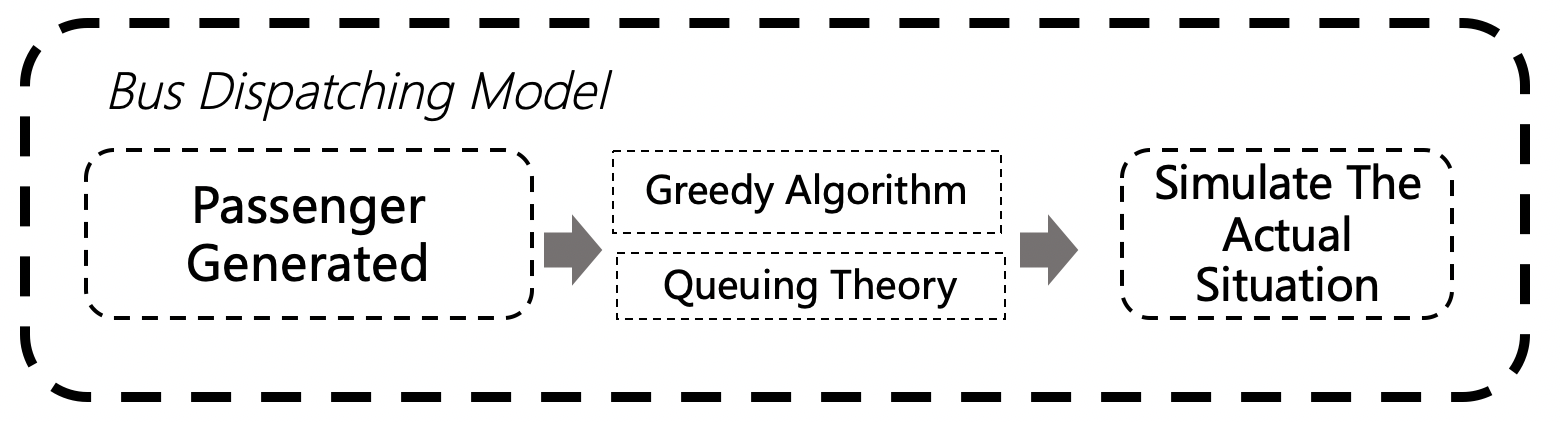
\includegraphics[width=0.8\textwidth]{figures/flowchart2.png}
    \caption{Flow Chart of Bus Dispatching Model}
    \label{fig:flowchart2}
\end{figure}
\subsubsection{Simulation of each passenger}\label{subsub:simu}

For each flight, we suppose the time people walk out of the airport is roughly in line with the normal distribution. This is reasonable, since the majority number of people walk out of the airport at the same time and only a few passengers come out early or late. Therefore, passengers-generated function is subject to normal distribution with multiple peaks.

For each passenger, we suppose that he uses our APP BusHub in the first place, as our service is cheap and timely. Within one minute, BusHub will respond whether there's a suitable bus for the user or not. As a result, he may choose other means to leave the airport, such as calling a taxi or stick to trying to book the next bus again. From the previous data, we assume the possibility of a passenger calling a taxi or riding on a shuttle bus is 7000/18000 and 1200/18000 respectively. If unfortunately, though, passengers failed to get on any of the vehicle mentioned above, they would have to wait for the platform to arrange another bus for them, as vividly shown in Section \ref{sec:impl}.

For each bus, it will be directly back when it arrives at the last station in the route or as soon as there is no passenger on the bus.

\subsubsection{Greedy Algorithm for Orders}

According to our cost function and the route acquired, the destination of each passenger is roughly average on each route. So there is barely such occasion that a bus is not filled up with passengers for a long duration. Moreover, due to the conditions met by the fifty stations we selected, there will not be such situation that the number of passengers in one station is much smaller than that in other stations, either. Therefore, our selected routes and stations are both relatively good, and extreme situation hardly occurs. Since the difference between different routes is not that large in the aspect of price, distance, and traffic, we use the greedy algorithm to determine which route each bus takes and which people to take practically.

As for our pricing strategy, we set the price for \textbf{each station} separately and adopted a hierarchical pricing strategy. This can facilitate user satisfaction, and reduce the spending of many passengers, which can be realized through BusHub conveniently. When it comes to the price function, it has something to do with distance and traffic conditions. The longer the distance, the the better the traffic condition, the lower the price is. In order to achieve a decent balance between revenue and user experience, we set the price function as a convex function of distance and traffic, shown in Equation \ref{pric}.


\begin{equation}\label{pric}
    Price=Max\, Price * \frac{\mathrm{ln} (1+ Population * Traffic)}{Max\, \mathrm{ln} (1+ Population * Traffic)}  
\end{equation}

Based on our price function, we mainly take into account bus drivers' salary, oil cost, management human cost, and vehicle maintenance cost, generating the profit function presented in Equation \ref{prof}.

\begin{equation}
    \begin{split}
     Profit &= Ticket + Advertisement\\ 
           &- Drivers' Wage - Oil - Management - Vehicle Maintenance  
    \end{split}
    \label{prof}
\end{equation}

\section{Implementation}\label{sec:impl}

\subsection{Data}
We successfully find a colorfully-pointed graph, which indicates the population density. $P(x,y)$ is generated through the graph. With knowledge and techniques in digital image processing, we use the population density assigned to each color and color distribution, as well as noise reduction methods to get the two-dimension mathematical function $P(x,y)$. $T(x,y)$ is acquired through the given data set. Form the given data set, we assign a limited value to each existing map point. We take the longitude, latitude, speed, and status(occupied) into account, after which we apply convolution techniques to relevant values in order to form a two-dimension mathematical function $T(x,y)$. There are two charts below in Figure \ref{fig:two}, showing the two function's distribution.

\begin{figure}[htbp]
    \begin{minipage}{0.44\linewidth}
      \centerline{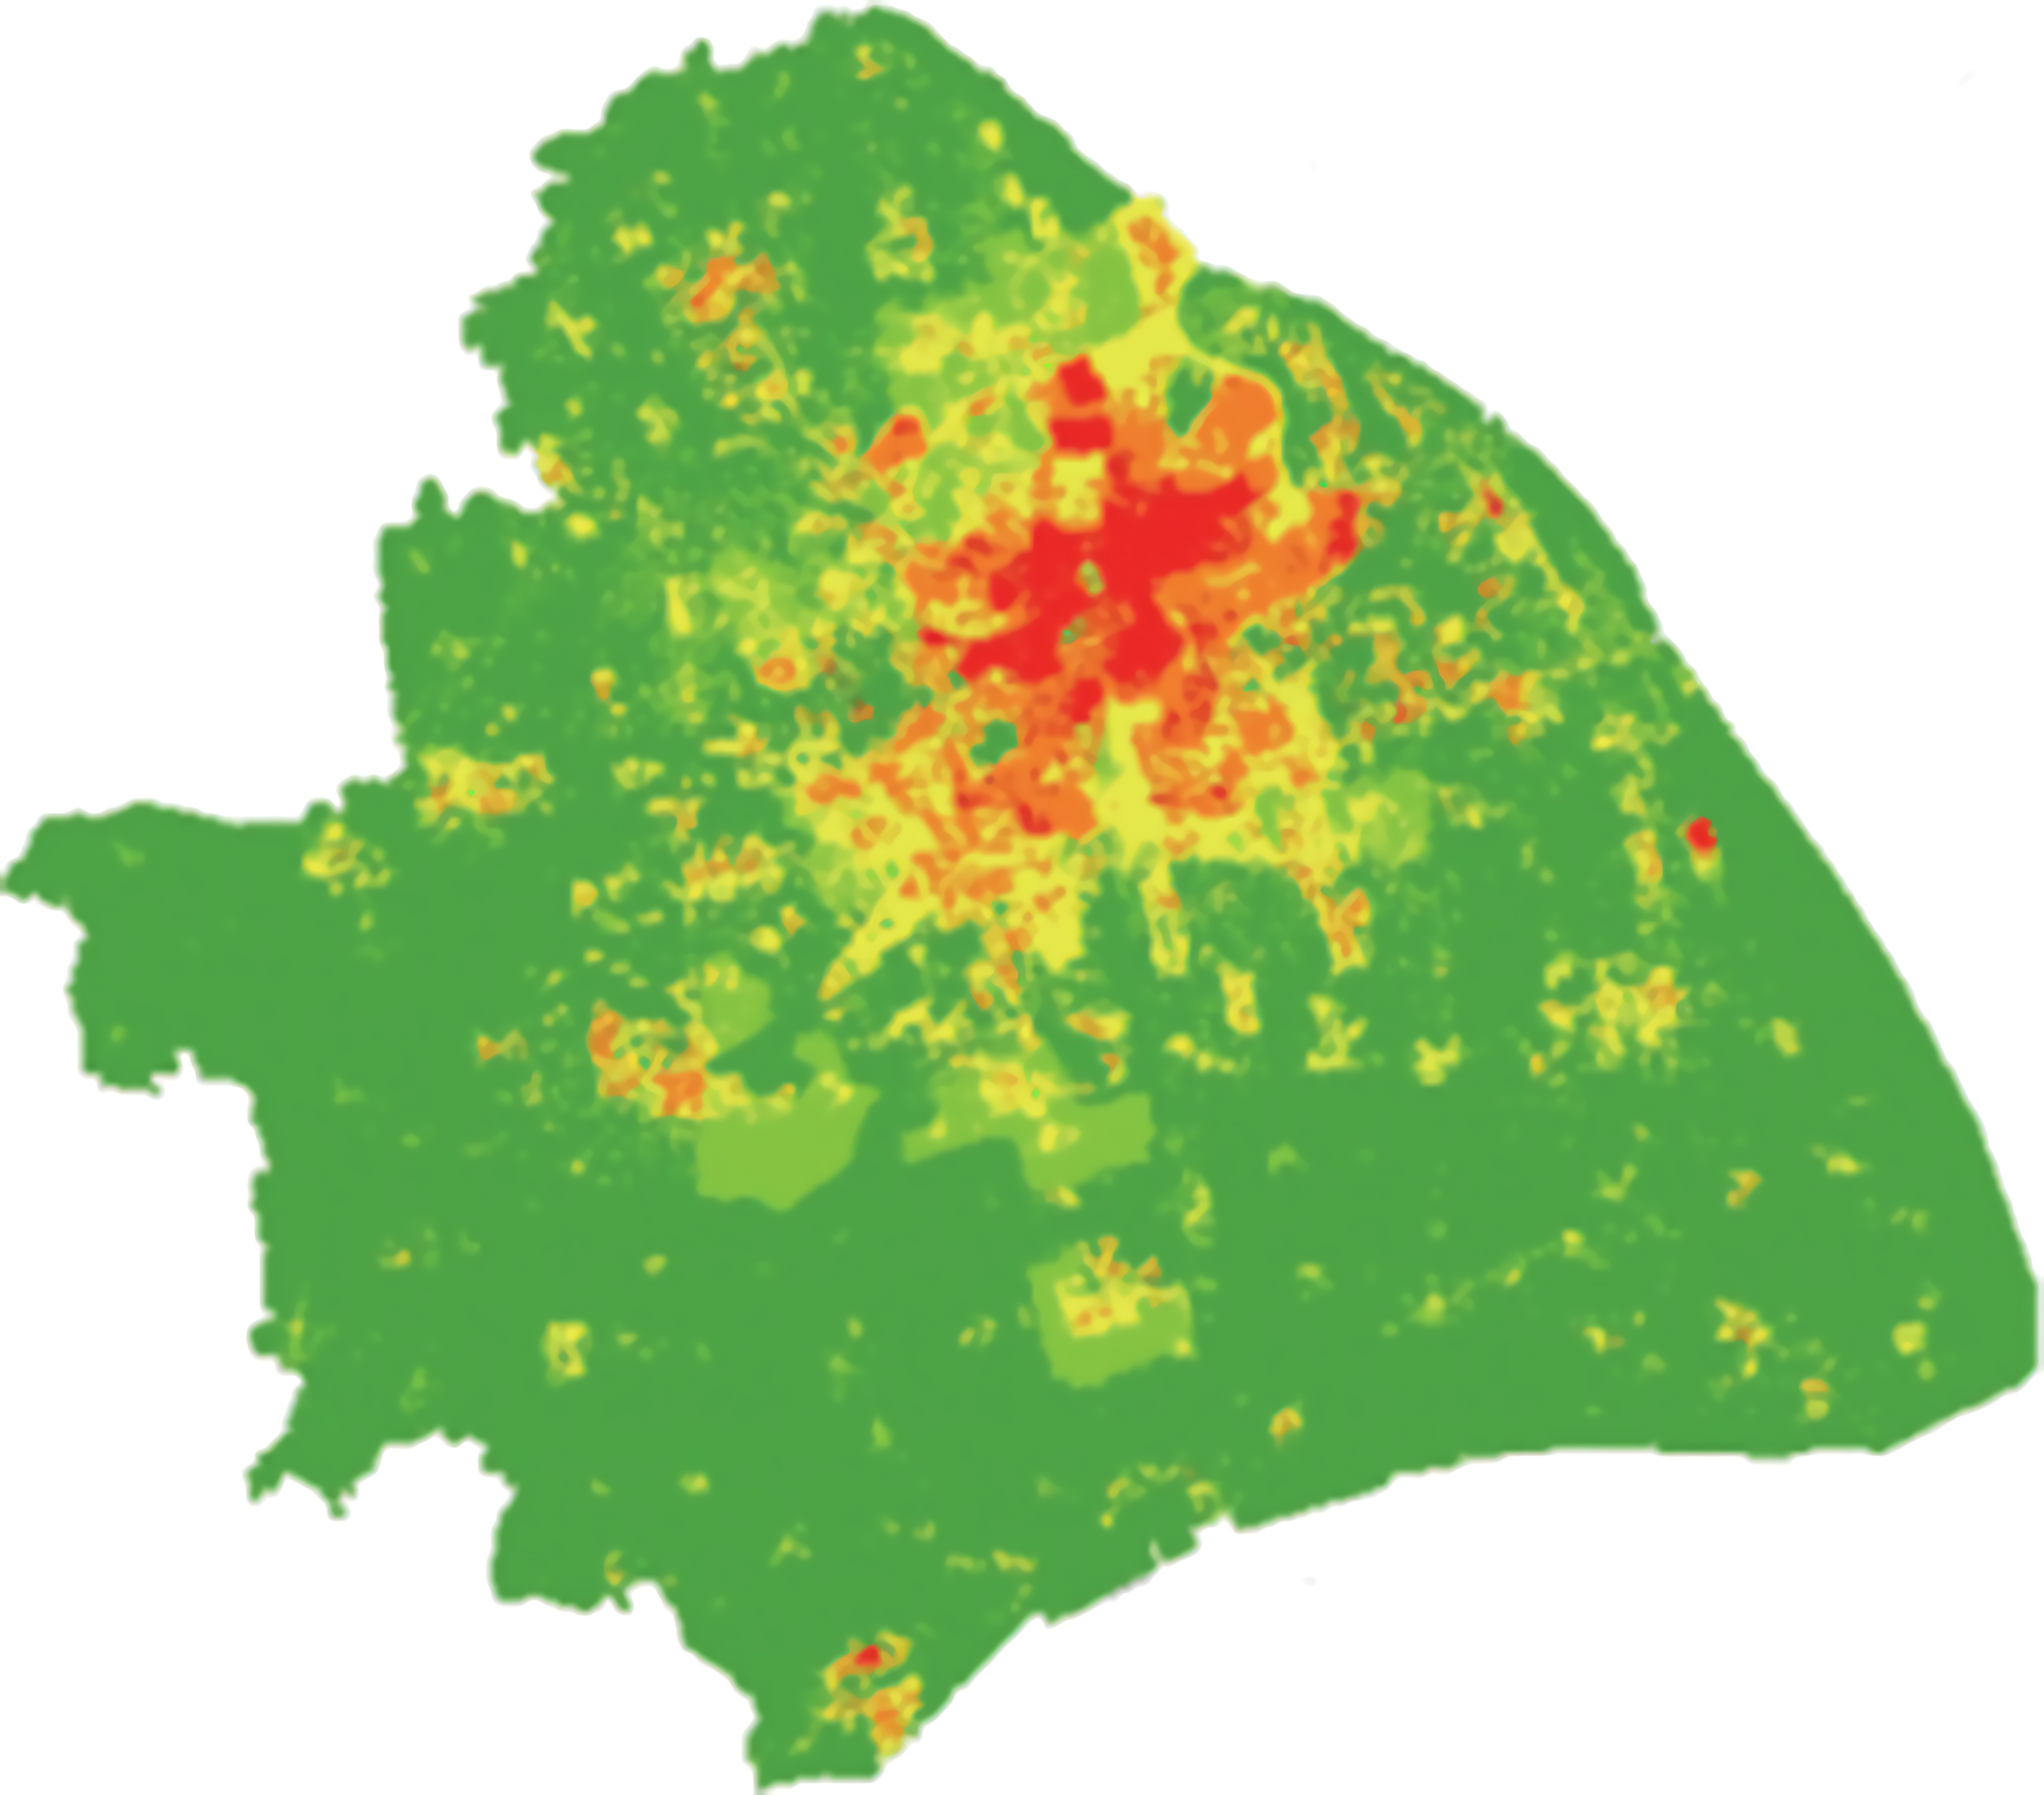
\includegraphics[height=6cm,width=7cm]{figures/Pd.jpg}}
      \caption*{(a) Population Density of Shanghai.}
      \cite{dqxxkx_ppl}
    \end{minipage}
    \hspace{0.5in}
    \begin{minipage}{0.44\linewidth}
      \centerline{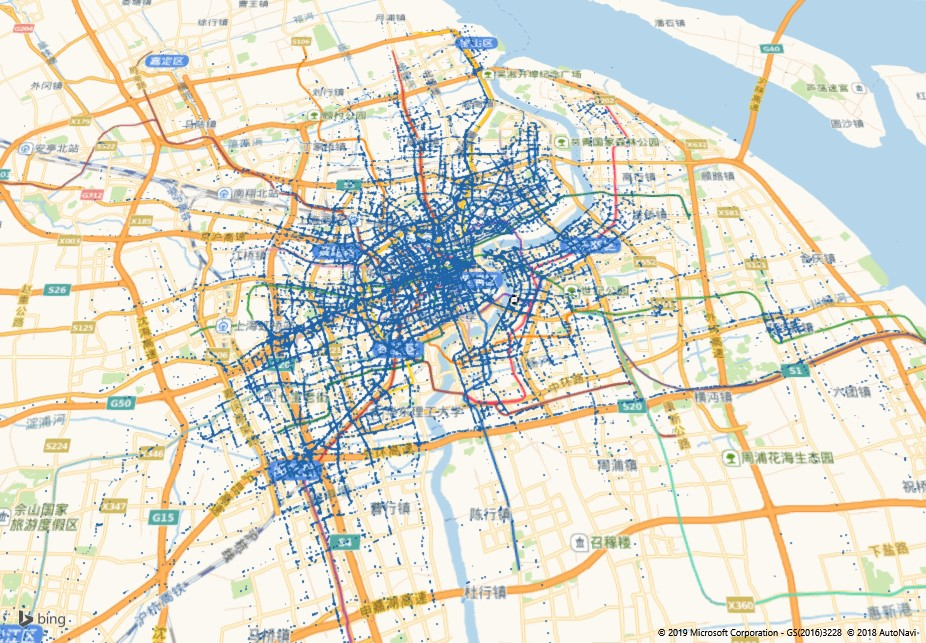
\includegraphics[height=6cm,width=7cm]{figures/Tran.png}}
      \caption*{(b) Traffic Density of Shanghai at midnight.}
    \end{minipage}
    \caption{In figure(a), a red point means higher population density, while a green point means lower; In figure(b), each blue point represents a GPS-recognized position. This means the denser the blue points are, the higher the traffic density.}
    \label{fig:two}
\end{figure}

\subsection{Outcomes of Model}

\subsubsection{Selected Destinations}
In order to get smooth function images of $P(x,y)$ and $T(x,y)$, Gaussian Low Pass Filter (GLPF)~\cite{DigitalImageProcessing} is applied to our sampling. The two-dimension version function of the filter is

\begin{equation}
    \begin{split}
      H(u,v)     & =   e^{-D^2(u,v)/2\sigma^2}\\
                 & =   e^{-9D^2(u,v)/2R^2}
    \end{split}
\end{equation}

where:
\begin{itemize}
\item $D(u,v)$ is the distance from the center of the frequency rectangle;
\item $\sigma$ is a measure of the degree of central expansion, which is equal to $\left( \frac{R}{3} \right)$;
\item $R$ is the precision radius, which is equal to 600 metres.
\end{itemize}

Then, we acquire a reasonable distribution of $M(x,y)$. Its picture is shown in Figure\ref{fig:M(x,y)}:

\begin{figure}[htbp]
    \centering
    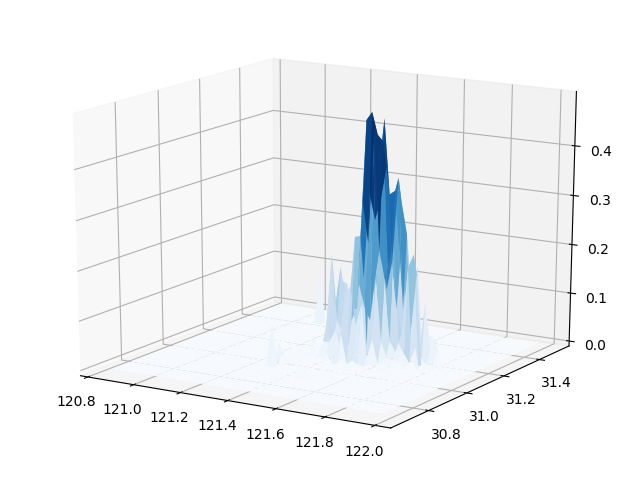
\includegraphics[width=10cm]{figures/M(x,y).png}
    \caption{Distribution of M(x,y)}
    \label{fig:M(x,y)}
\end{figure}

Afterwards, we use the Destination Selection Model and Route Selection Model to generate one thousand \textbf{potential destinations}, and finally integrate them into \textbf{fifty destination stations}. These two steps are depicted in Figure \ref{fig:twoII}.

\begin{figure}[htbp]
    \begin{minipage}{0.44\linewidth}
      \centerline{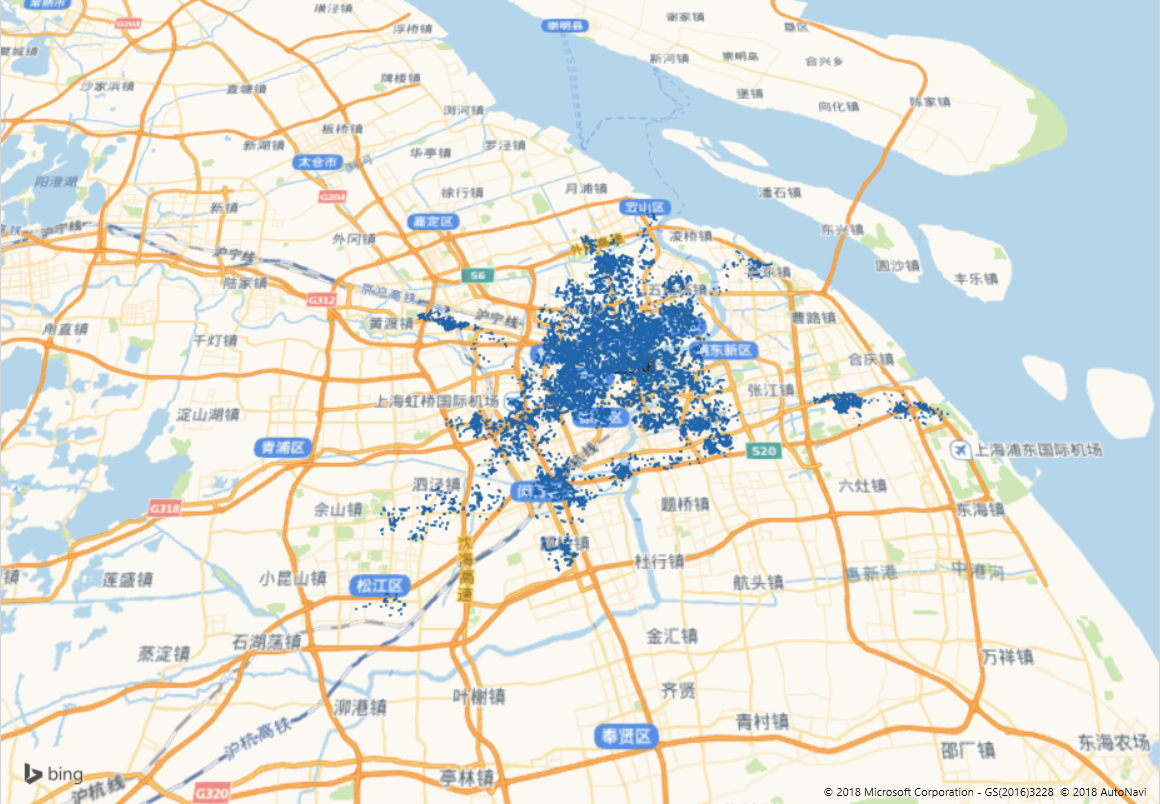
\includegraphics[height=5cm,width=7cm]{figures/PotentialDetinations.png}}
      \caption*{(a) Distribution of Potential Destinations.}
    \end{minipage}
    \hspace{0.5in}
    \begin{minipage}{0.44\linewidth}
      \centerline{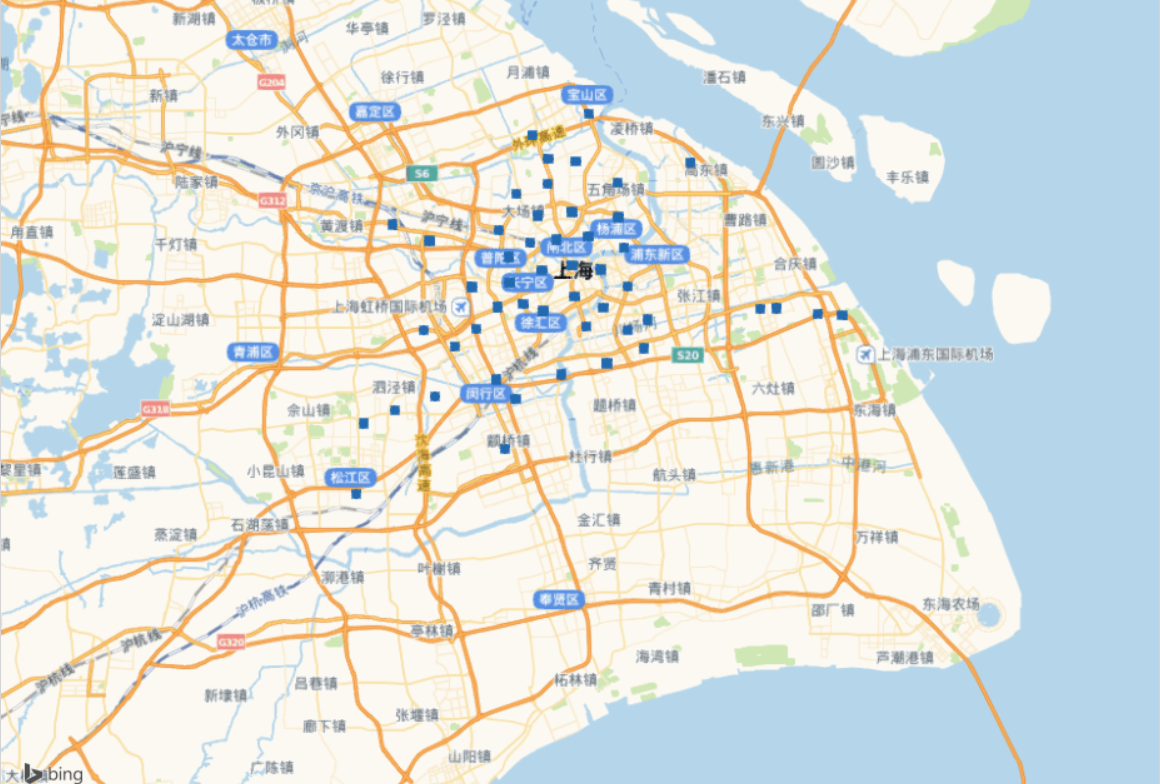
\includegraphics[height=5cm,width=7cm]{figures/fiftydestinations.png}}
      \caption*{(b) Distribution of fifty Destinations.}
    \end{minipage}
    \caption{Generation of fifty Destinations}
    \label{fig:twoII}
\end{figure}




We turn the destination address from the longitude-latitude form to detailed text address in Chinese. Thus, the APP can be more user-friendly. We extract a part of the total destinations shown in Figure\ref{fig:AIC}. All destinations are clearly set out in the appendix.

\begin{figure}[htbp]
    \centering
    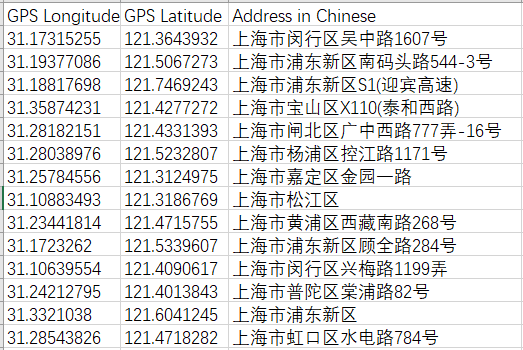
\includegraphics[width=8cm]{figures/AddressinChinese.png}
    \caption{Part of the Destinations' Addresses in Chinese}
    \label{fig:AIC}
\end{figure}

\subsubsection{Selected Routes}

\begin{figure}[htbp]
    \begin{minipage}{0.45\linewidth}
      \centerline{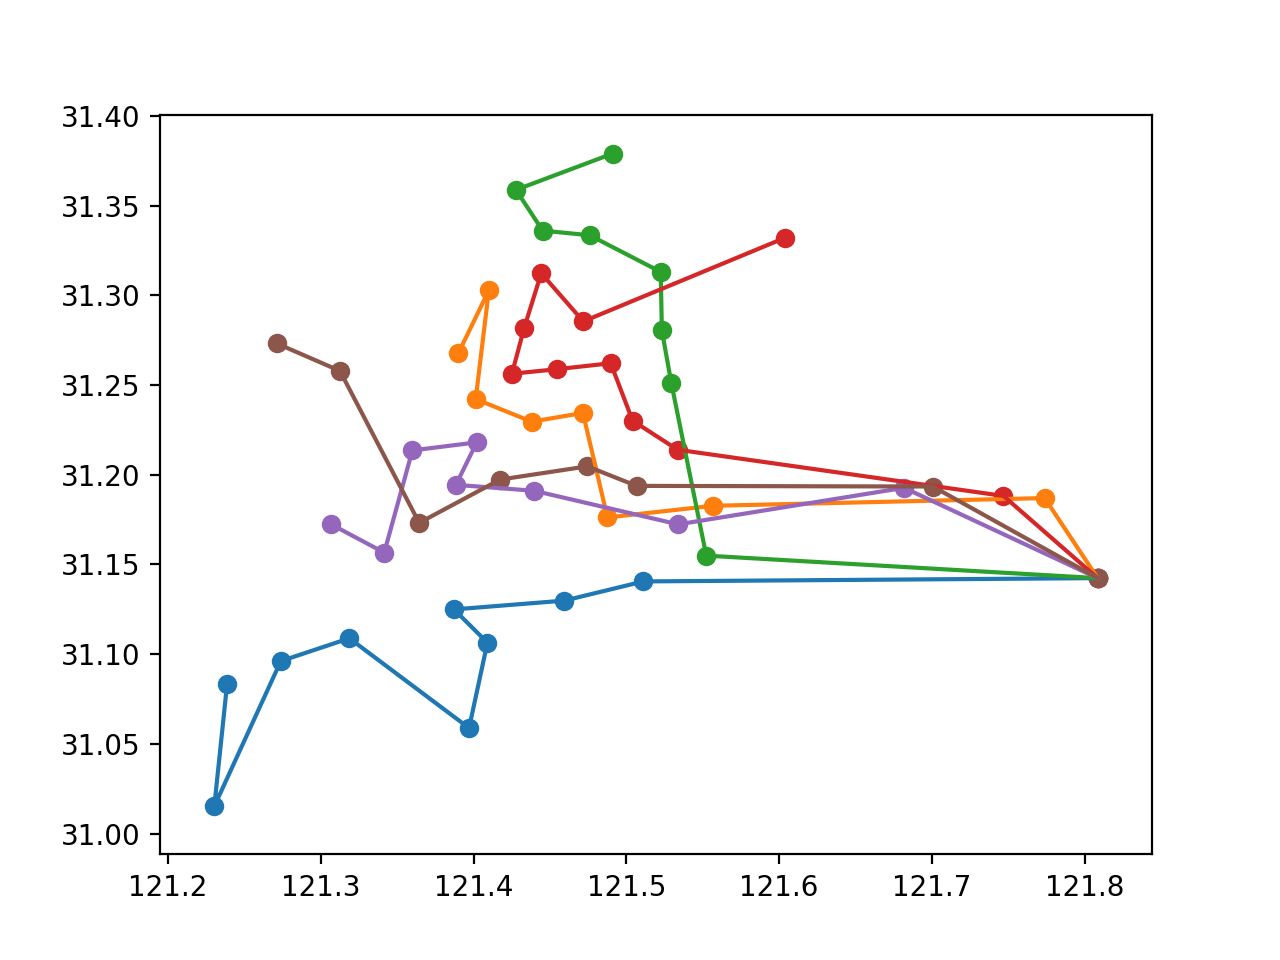
\includegraphics[width=8cm]{figures/6routesprime.png}}
      \caption*{(a) Six model-generated routes}
    \end{minipage}
    \hspace{0.5in}
    \begin{minipage}{0.45\linewidth}
      \centerline{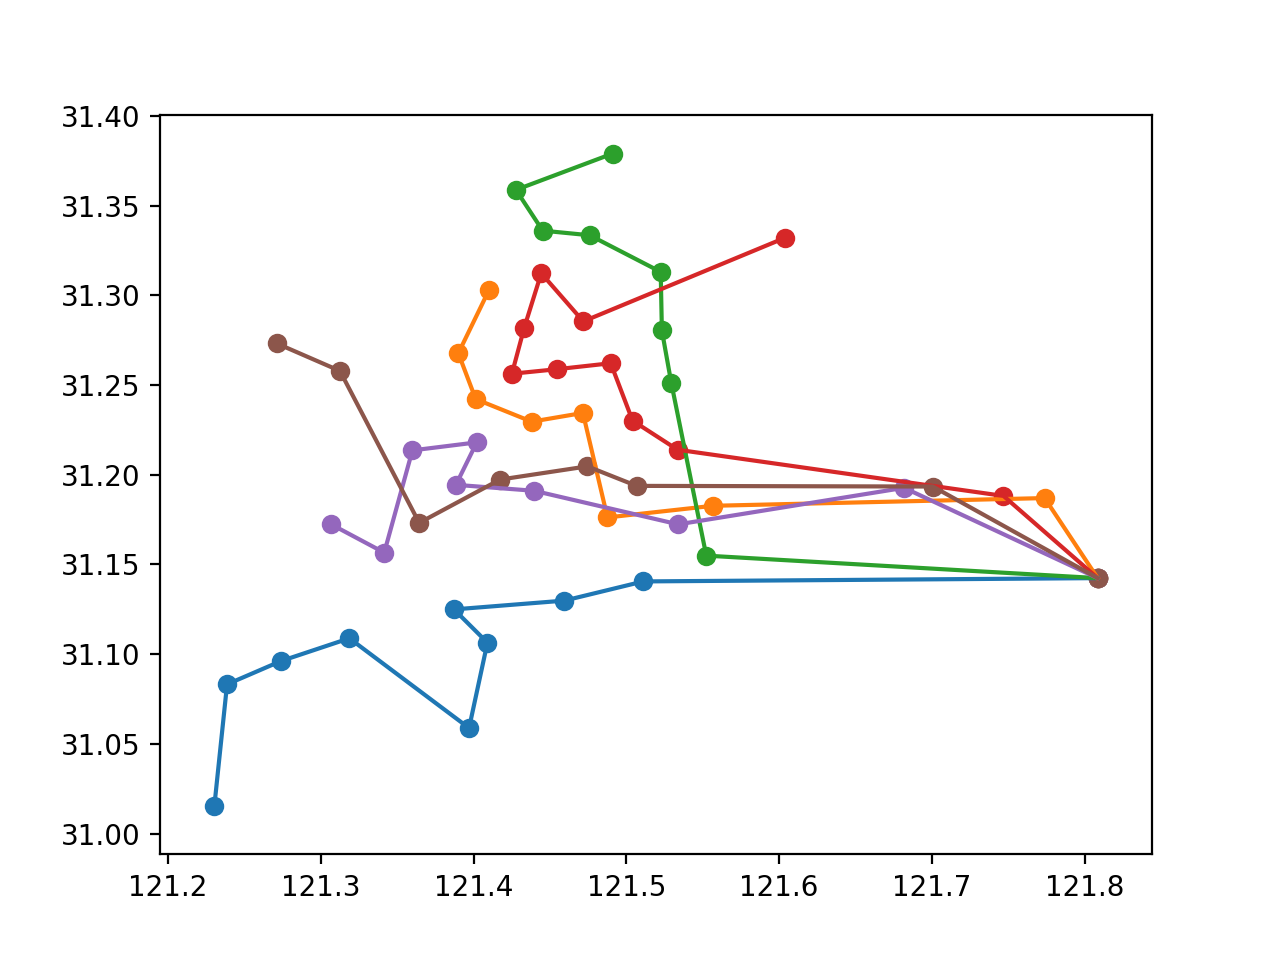
\includegraphics[width=8cm]{figures/6routes.png}}
      \caption*{(b) Six model-generated routes after human intervention}
    \end{minipage}
    \caption{Generation of six Routes}
    \label{fig:routes}
\end{figure}
Since destinations are chosen, we can now plan our routes with Simulated Annealing. Here we set number of routes $N_R$ to be 6, the reason of selecting this number will  be analyzed in next section. At the same time, we set $N_{cand}$ to be 2. As for SA parameters,  since our computers are not so high-powered, we set initial temperature $T=0.5$, minimum temperature $T_{min}=0.05$ and number of iterations in every temperature $N_{iter}=10$. The results are demonstrated in Figure \ref{fig:routes}. Note that the last two edges of blue and the orange route seems twisted. This two routes may have lower costs, but make it contradicts to the general perception of a typical bus line. So we fix this two small edges through human intervention. The final output is shown in Figure \ref{fig:routes}(b).

\subsubsection{Simulation of Passengers}

As mentioned in Section \ref{subsub:simu}, we simulate the passengers' arrival at the starting station. Considering the total number of people to be transported, reasonable price and profits, and shorter waiting duration, we set the number of buses from BusHub a hundred and fifty, and get the following outcomes.
\begin{table}[h]
    \centering
    \caption{Outcomes of an optimized simulation}
    \label{tab:simu}
    \linespread{1.5}
    \begin{tabular}{c c c}
\hline
    	Items & Outcomes & Units\\
\hline
	$The\, Number\, of\, Bus$ & 150 & / \\
	$The\, Number\, of\, Passengers\, Taking\, Taxi\, and\, Bus$ & 8,146 & ppl \\
	$The\, Number\, of\, People\, Carried\, by\, BusHub$ & 9,603 & ppl \\
	$Total\, Profits$ & 70,139 & RMB \\
	$The\, Average\, Waiting\, Time$ & 10.420 & min \\
\hline
    \end{tabular}
\end{table}

As shown in Figure \ref{150}, in the left side of the horizontal axis
, many passengers who arrive at around 20 minutes need some time to wait. This is because the occupancy rate has to reach a certain rate for each bus to depart. Otherwise, it is a waste of limited resources. Then a peak waiting time comes, when BusHub runs out of all buses, so passengers need to wait until the buses come back. 

\begin{figure}[htbp]
    \centering
    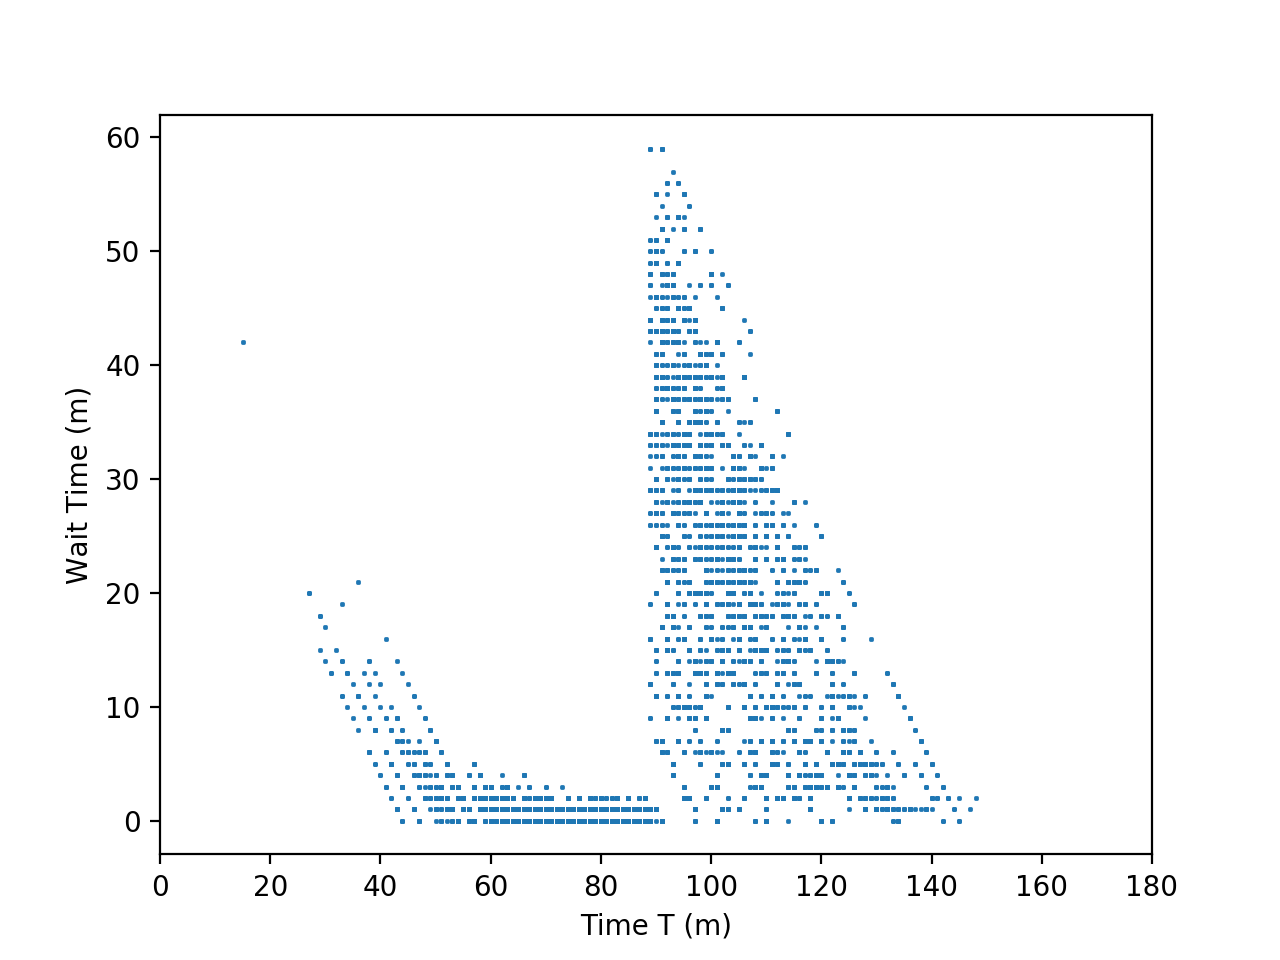
\includegraphics[height=8.5cm,width=16cm]{figures/waittime150.png}
    \caption{Wait Duration - Time passengers arrive at the starting station}
    \label{150}
\end{figure}

The model achieve a great balance between these items, and can suits the actual situation.

\begin{figure}[htbp]
    \centering
    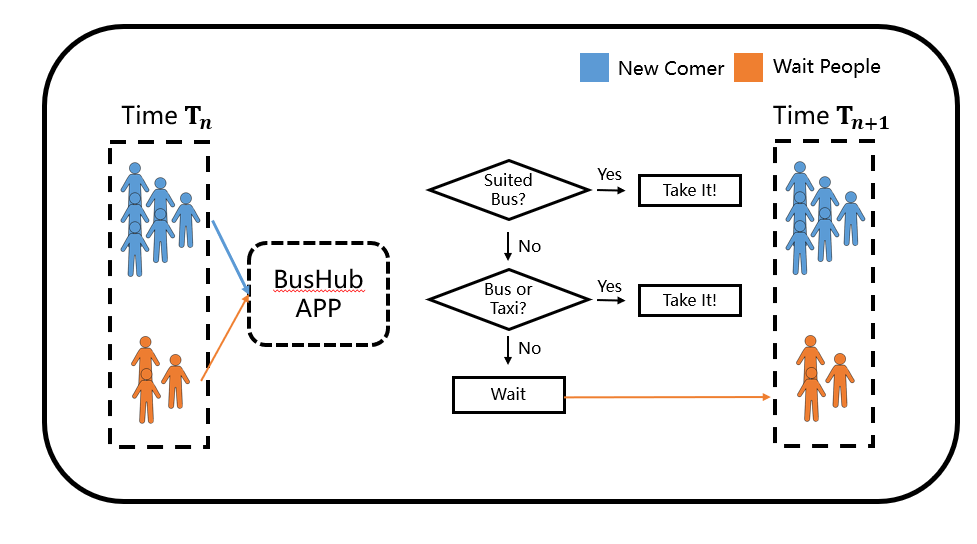
\includegraphics[height=8.5cm,width=16cm]{figures/APP.png}
    \caption{How BusHub works}
    \label{fig:BusHub}
\end{figure}

Based on the three main models mentioned above, the bus-booking platform is integrated as a newly-released APP \text{BusHub} to meet customers' demands. BusHub receive orders, calculate backstage, and send feedbacks within one minute. In order to promote customer loyalty and user satisfaction, BusHub goes to great lengths to satisfy as many orders and as little waiting time as possible. The diagram in Picture \ref{fig:BusHub} shows how it works.


\section{Model Analysis}\label{sec:mode}

\subsection{Sensitivity Analysis}
Our models contain several parameters. We determine some of the parameters through AHP, digital image, some of them by knowledge in the article or other methods. In the following section, we would like to produce a sensitivity analysis to show whether our model is sensitive to different values of parameters.

\subsubsection{Bus Number}
\begin{figure}[htbp]
    \centering
    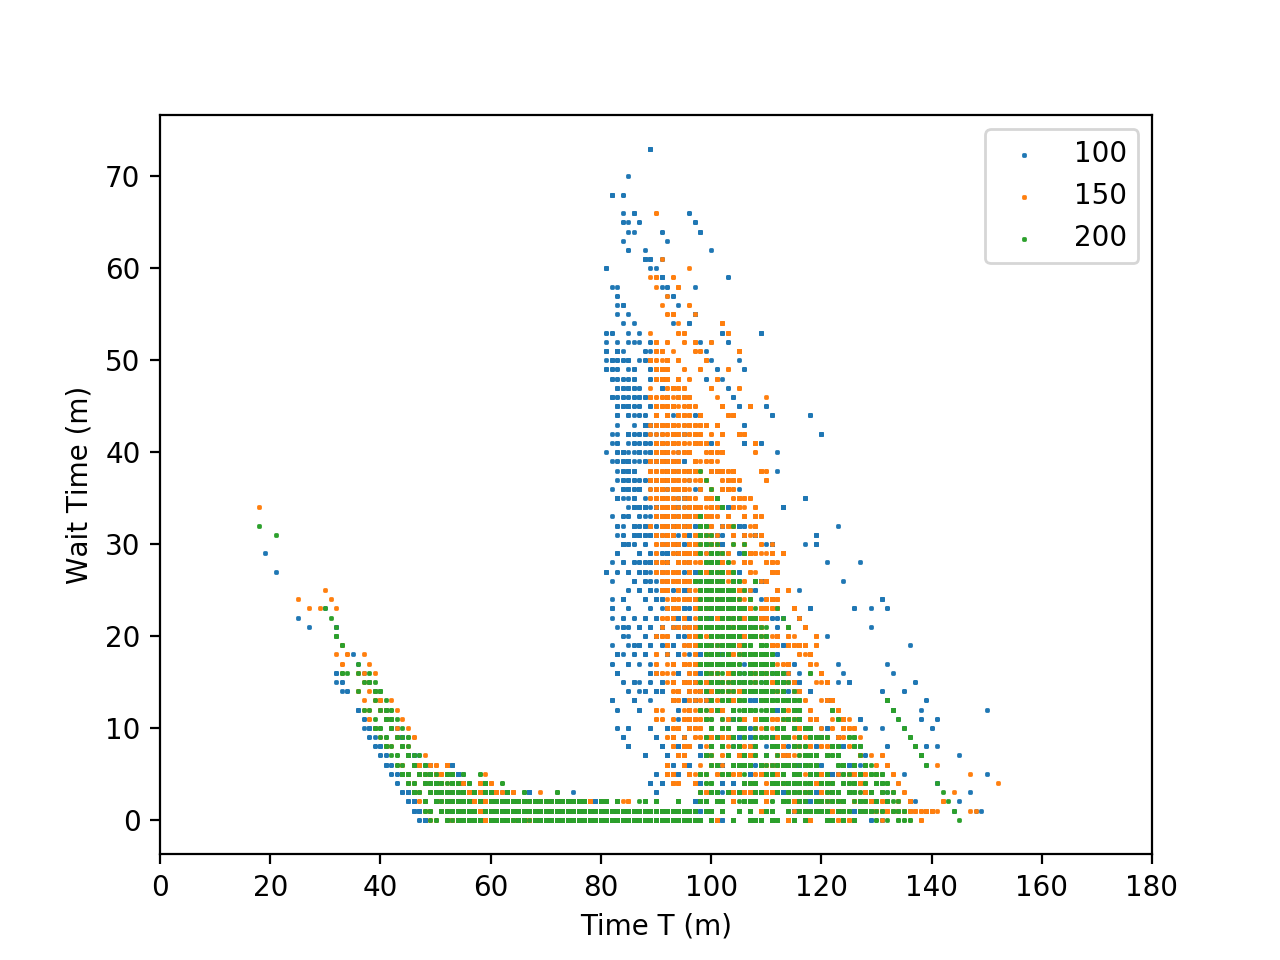
\includegraphics{figures/waittime.png}
    \caption{Wait Duration - Time passengers arrive at the starting station figure for different number of buses.}
    \label{fig:waittime}
\end{figure}

\begin{table}[h]
    \centering
    \caption{Outcomes of Different Number of Buses}
    \label{tab:outc}
    \linespread{1.5}
    \begin{tabular}{cccc} 
\toprule
Bus Number & 100 & 150 & 200\\
\midrule
Passengers Taking Taxi and Shuttle Bus & 8278 & 8146 & 8130 \\
Passengers carried(ppl) & 6897 & 9603 & 9768 \\
Profits(RMB) & 52635 & 70139 & 61784 \\ 
Average Waiting Time(min) & 12.294 & 10.420 & 3.685 \\
\bottomrule 
\end{tabular}
\end{table}

As shown in Table \ref{tab:outc} and Figure \ref{fig:waittime}, if there are more buses, we can pick up more passengers and reduce passengers' average waiting time. However, more buses lead to higher fundamental cost, which deduct BusHub profits, show in line three in Table \ref{tab:outc}.

According to the profit function\ref{prof}, we , and then draw a conclusion that about 150 buses satisfy peak period's need. But this may cause waste in the daytime.

\subsubsection{Routes Number}

\begin{figure}[htbp]
    \begin{minipage}{0.44\linewidth}
      \centerline{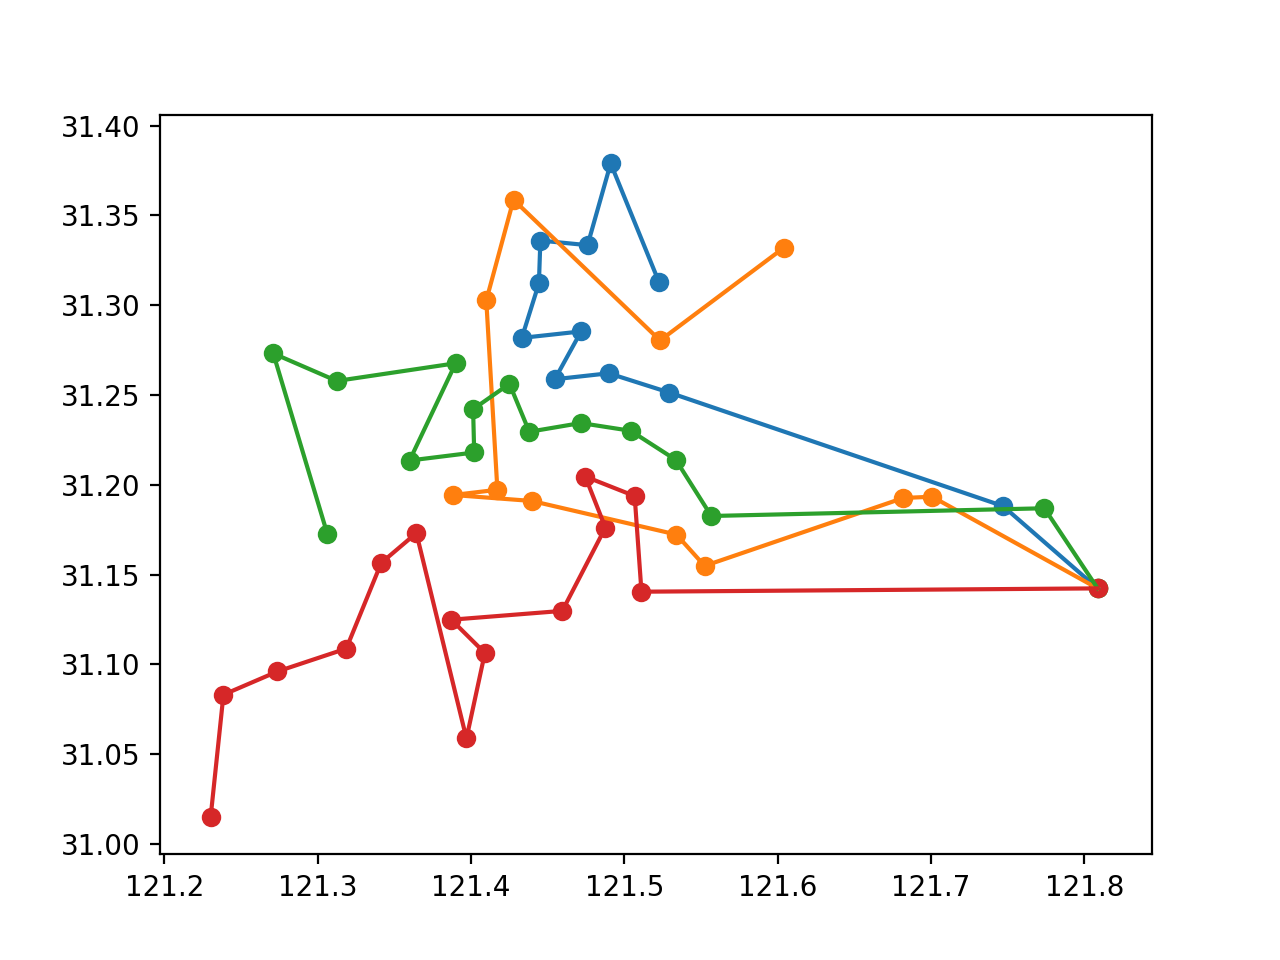
\includegraphics[height=6cm,width=7cm]{figures/4routes.png}}
      \caption*{(a) 4 Routes.}
    \end{minipage}
    \begin{minipage}{0.44\linewidth}
      \centerline{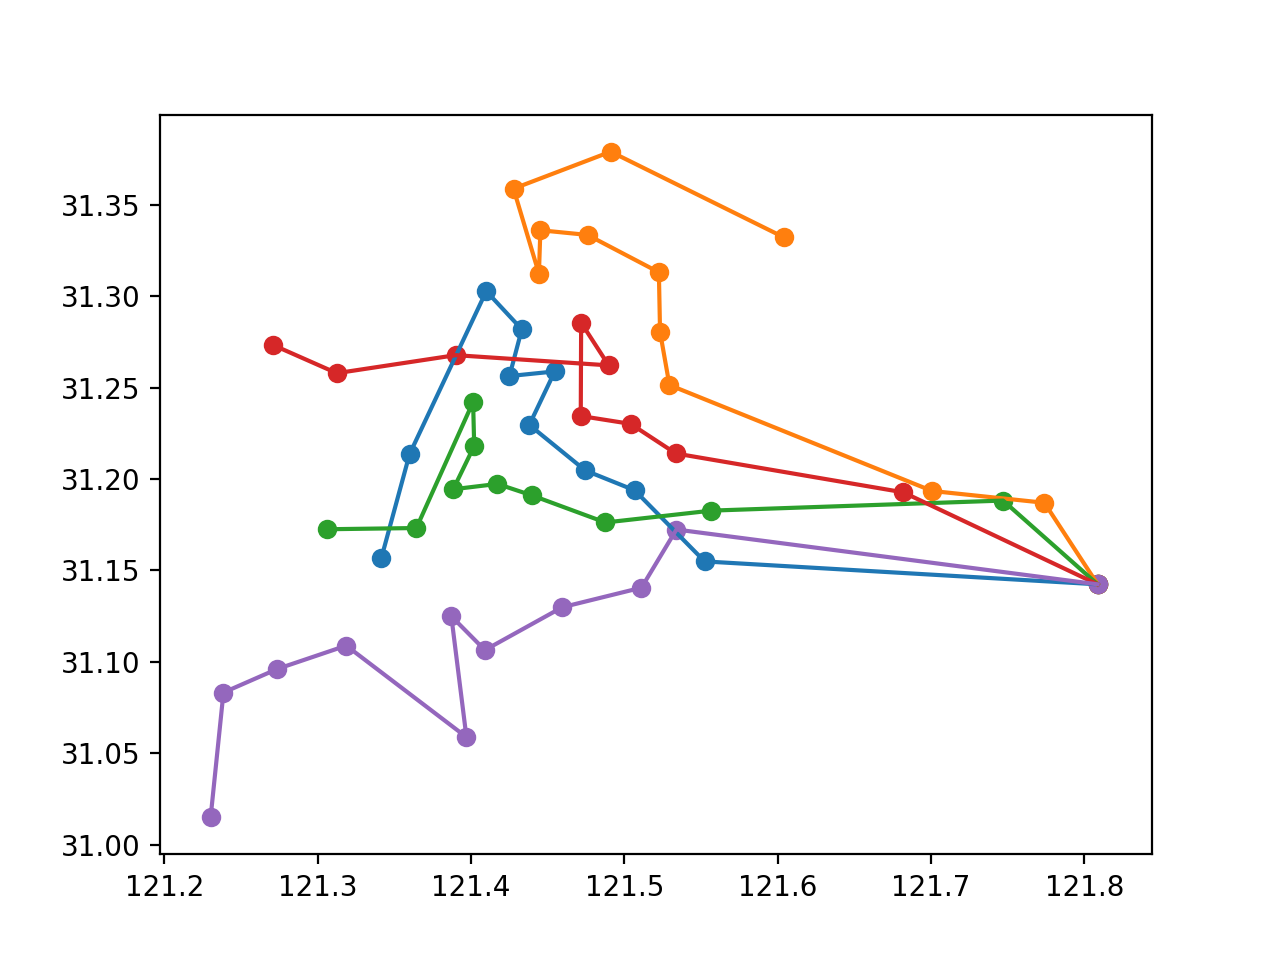
\includegraphics[height=6cm,width=7cm]{figures/5routes.png}}
      \caption*{(b) 5 Routes.}
    \end{minipage}
    \begin{minipage}{0.44\linewidth}
      \centerline{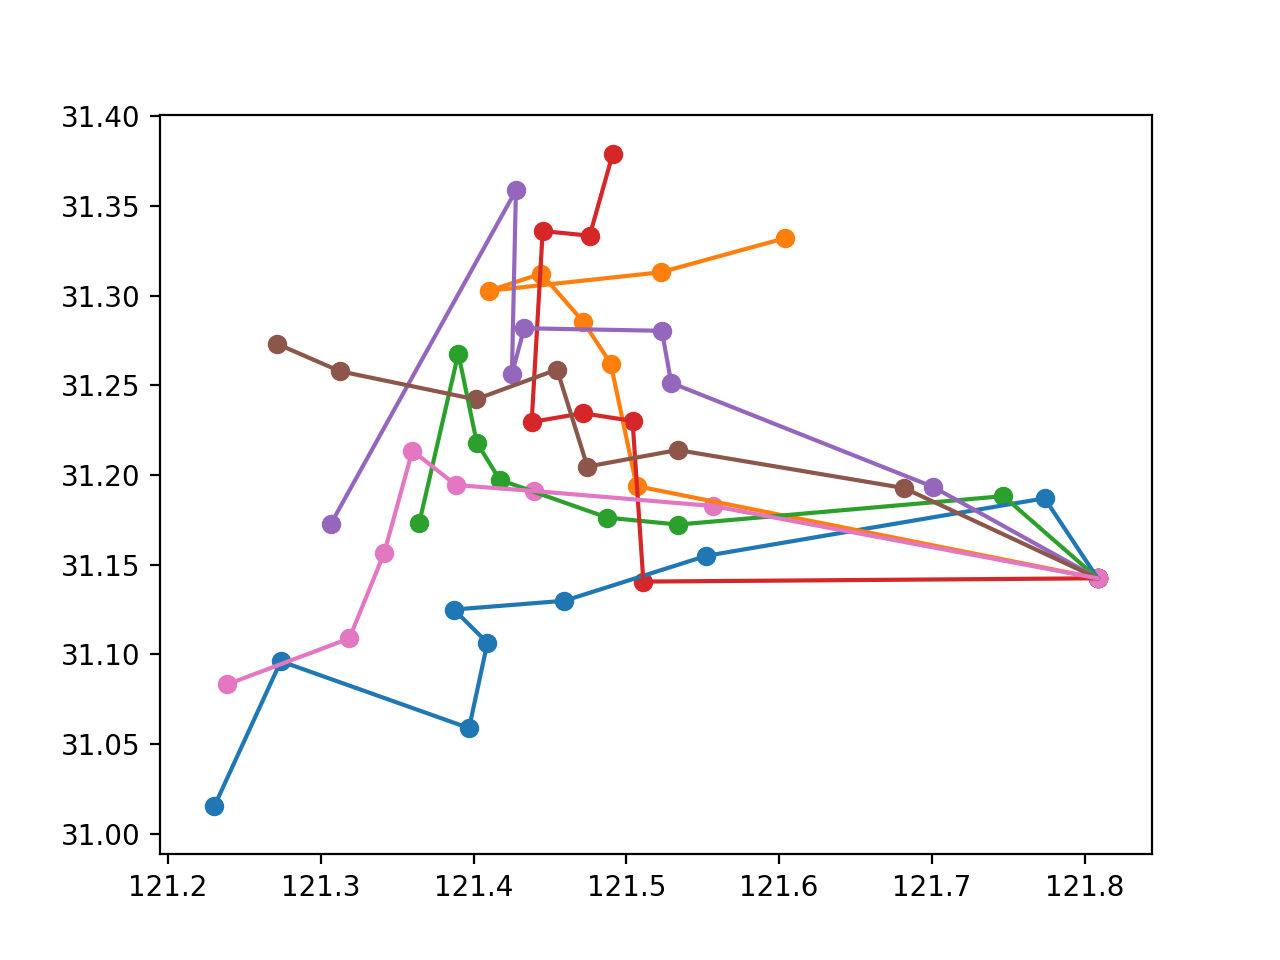
\includegraphics[height=6cm,width=7cm]{figures/7routes.png}}
      \caption*{(c) 7 Routes.}
    \end{minipage}
    \hspace{0.7in}
    \begin{minipage}{0.44\linewidth}
      \centerline{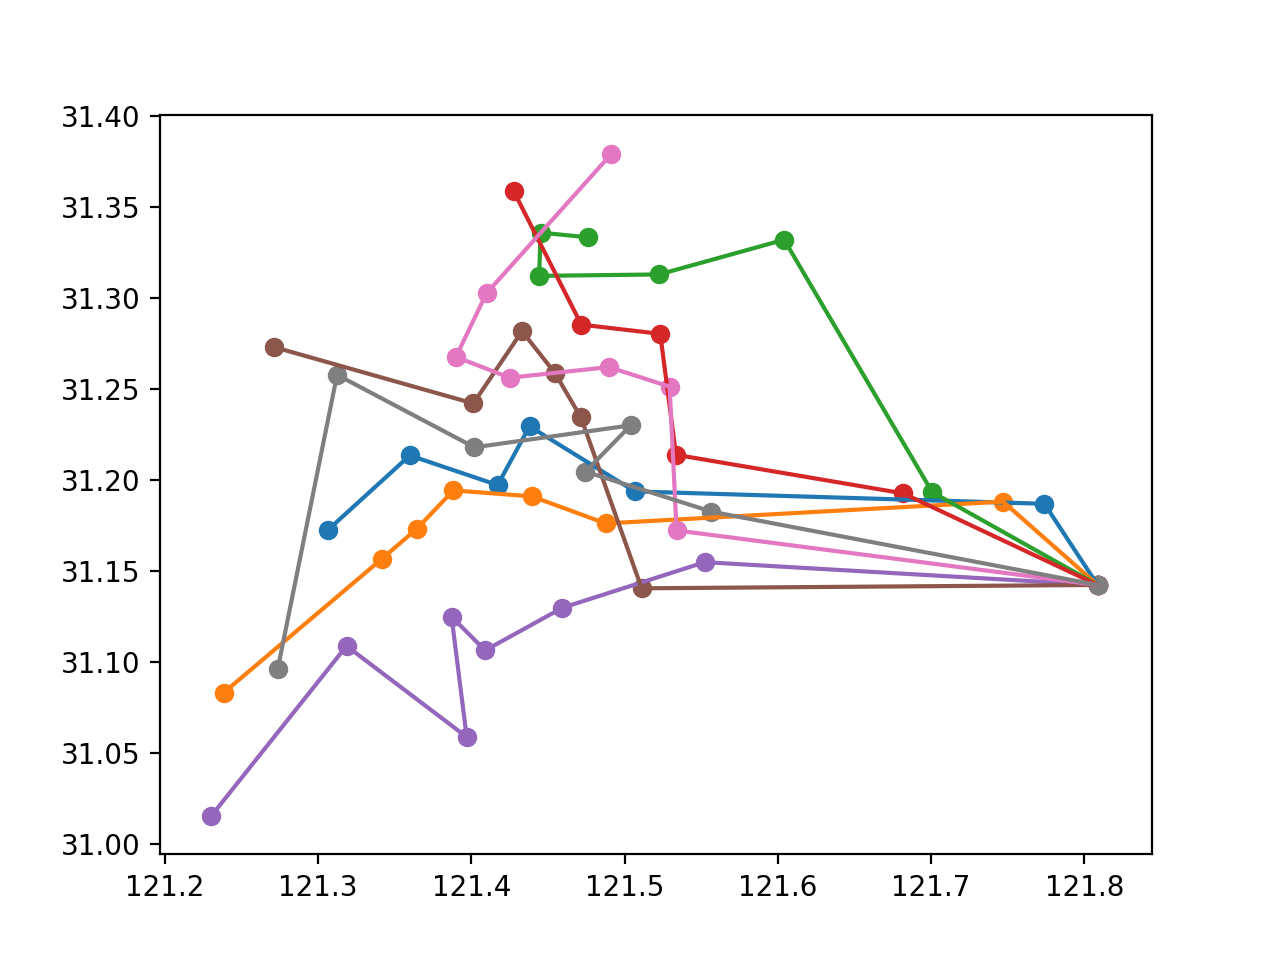
\includegraphics[height=6cm,width=7cm]{figures/8routes.png}}
      \caption*{(d) 8 Routes.}
    \end{minipage}
    \caption{Different Routes Numbers' Result}
    \label{diffroutes}
\end{figure}

According to the routes as shown in Figure \ref{diffroutes}, if there are five or less routes, passengers diversified demands are not met properly; if there are more than six routes, different routes are quite similar to each other, which is obviously a waste of our existing transport capacity.

\subsubsection{AHP Parameter}
In Section \ref{ahp_tab}, we assign different values to each coefficient. In our model analysis, we change the values of coefficient, and receive similar results.

\subsection{Strengths and Weaknesses}
\subsubsection{Strengths}
\begin{enumerate}
    \item We have reasonable and accurate sources of data, and our model is logically rigorous. During our brainstorm, we come up with many tough conditions, and revise the generated model to be more user-friendly.
    \item We adopt interdisciplinary methods in our model. Color channel analysis and Gaussian Low Pass Filter are wide adopted in Digital Image Processing. We borrow these methods to aid our model.
    \item Our model is highly practial. All the theories in our model are concretely implemented and we offer comprehensive analysis and discussion of the results.
    \item We use fancy visualization and clear diagram to state our model.
    \item We make great effort in brand design of our app BusHub, including the name, the logo and the poster, which are sure leave our customers a fresh impression.
\end{enumerate}


\subsubsection{Weaknesses}
\begin{enumerate}
    \item Straight-line distance is used in our model. However, actual situation is more complex and tough. Spherical distance and Manhattan is more precise. 
    \item More real-life situations should be taken into account, such as real-time traffic conditions, and traffic density differences between day.
    \item Passengers' advice is important, too. Their opinion on route and destination selection also matters.
\end{enumerate}

\section{Conclusion}\label{sec:conc}

Our paper provides a detailed solution of enabling most people off the red-eye flights yo arrive at their destinations \textbf{without waiting for a long duration}. We come up functions to quantify the profits and user satisfaction. Our integrated model consists of three models, namely Destination Selection Model, Route Selection Model, and Bus Dispatching Model. We use the profit and our three model to keep a balance between maximizing BusHub's profits and minimizing passengers' waiting time.

We use different sources of data to instantiate our model, and give a proper recommendation as to the number of buses, selected destinations, and routes.

Model Analysis are fully discussed to explain why we choose that set of statistics to run our app BusHub. There's also a delicate advertisement in the next section, showing how to use BusHub.

\newpage\label{page}
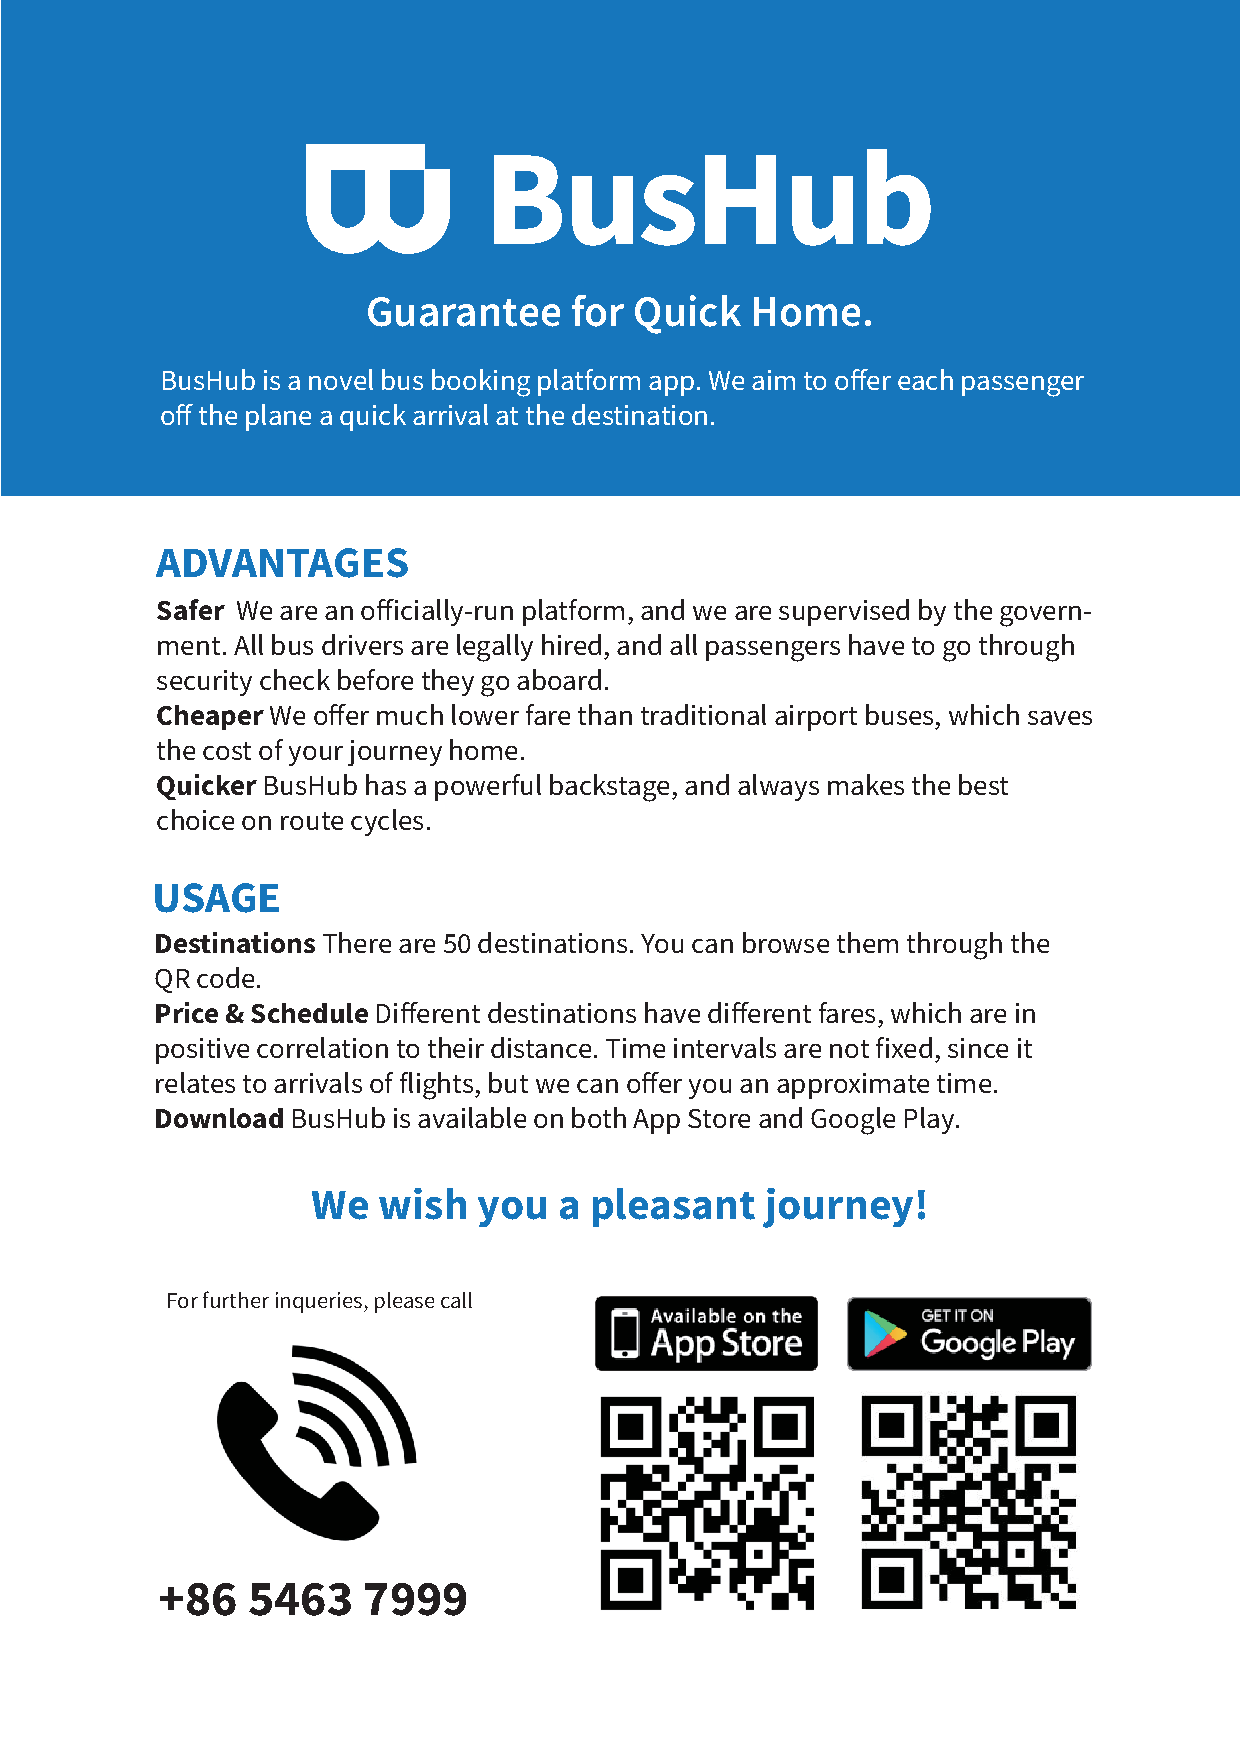
\includepdf[pages={1}]{ad.pdf}

\section{Advertisement}\label{sec:adve}
Our advertisement is shown upward in Page \ref{page}.

\bibliographystyle{IEEEtran}
\bibliography{newrefs}

\newpage
\begin{appendices}
\section{Fifty Selected Destinations}
% Table generated by Excel2LaTeX from sheet 'Stations'
\begin{table}[htbp]
  \centering
  \caption{Longitude and Latitude of Fifty Destinations}
  \renewcommand\arraystretch{1.35}
    \begin{tabular}{|c|c|}
    \multicolumn{2}{c}{Fifty Destination Stations} \\
    \hline
    Longitude & Latitude \\
    \hline
    121.364393162531  & 31.173152552460  \\
    121.506727261692  & 31.193770863610  \\
    121.746924348685  & 31.188176982499  \\
    121.427727151510  & 31.358742313098  \\
    121.433139324850  & 31.281821514808  \\
    121.523280704171  & 31.280389760460  \\
    121.312497485300  & 31.257845558004  \\
    121.318676931596  & 31.108834932138  \\
    121.471575456181  & 31.234418142819  \\
    121.533960720319  & 31.172326196662  \\
    121.409061703513  & 31.106395542063  \\
    121.401384292276  & 31.242127947224  \\
    121.604124514158  & 31.332103796933  \\
    121.471828168427  & 31.285438256653  \\
    121.230262324458  & 31.015230791544  \\
    121.700675726468  & 31.193410339600  \\
    121.238600547066  & 31.083179839898  \\
    121.489783526947  & 31.262117133953  \\
    121.402093037180  & 31.218021052389  \\
    121.438025579592  & 31.229559793646  \\
    121.459520619477  & 31.129833350839  \\
    121.271084910573  & 31.273177521576  \\
    121.445246934034  & 31.336013691238  \\
    121.529393896826  & 31.251364350760  \\
    121.387172859152  & 31.124929047336  \\
    121.439640469256  & 31.191039080854  \\
    121.306396260030  & 31.172488372549  \\
    121.476011627950  & 31.333448666715  \\
    121.397037102902  & 31.058798512089  \\
    121.522513215793  & 31.313030242158  \\
    121.454646336302  & 31.258801946350  \\
    121.487640064119  & 31.176185161081  \\
    121.388412091579  & 31.194354995338  \\
    121.390018516950  & 31.267699508414  \\
    121.341503761017  & 31.156572158483  \\
    121.556704519879  & 31.182669427071  \\
    121.773870135207  & 31.186969896870  \\
    121.552350935580  & 31.154895396208  \\
    121.273777676284  & 31.096099848443  \\
    121.425089224955  & 31.256263202675  \\
    121.409972105050  & 31.302694807414  \\
    121.359945503646  & 31.213554954933  \\
    121.504103558526  & 31.230112052397  \\
    121.444298701623  & 31.312259258587  \\
    121.417223173704  & 31.197270242250  \\
    121.511163311648  & 31.140525418237  \\
    121.533558672333  & 31.213915495691  \\
    121.681836497288  & 31.192687075444  \\
    121.474509588538  & 31.204650653065  \\
    121.491086492494  & 31.378981942682  \\
    \hline
    \end{tabular}%
  \label{tab:addlabel}%
\end{table}%

\newpage
\section{Implemented Algorithms and Codes}
\subsection{Metropolis Hastings \& Simulated Annealing Algorithm}
\lstinputlisting[language=python]{mtr.py}

\subsection{Population Density Estimate}
\lstinputlisting[language=python]{pop.py}

\subsection{Transportation Density Estimate}
\lstinputlisting[language=python]{traf.py}

\subsection{Destination Stations Selection}
\lstinputlisting[language=python]{stt.py}

\subsection{Route Selection}
\lstinputlisting[language=python]{rt.py}

\subsection{Simulation of each passenger}
\lstinputlisting[language=python]{simulation.py}
\end{appendices}
\end{document}


